\chapter{Dataanalyse}
I denne fasen analyseres dataene som er samlet inn, og ved hjelp av statistiske verktøy kan vi trekke konklusjoner basert på svarene. I analysen kommer vi hovedsaklig til å bruke verktøy som er beskrevet i metodeboken \cite{RCA}, men vi har også benyttet oss av statistiske verktøy som kan gå dypere, men som ikke er like visuelt fremstillende. Etter denne fasen ønsker vi å sitte igjen med en mengde mulige årsaker til at NTNU sine kontoer blir kompromittert. Verktøyet vi har brukt til å utføre mesteparten av analysene er SPSS, et statistisk verktøy for å blant annet gjøre grafiske- og matematiske beregninger på et datasett.

\section{Ønsket utbytte}
Her beskrives det ønskede utbytte av de forskjellige verktøyene som er benyttet i analysefasen og hva vi bruker de til.

\subsection{Histogram}
Ved å benytte histogram håper vi å få en visuell fremstilling av data som gjør det raskt og enkelt å forstå disse, og derfor lettere kunne trekke konklusjoner. Disse blir stort sett brukt for å få en oversikt over svarprosent på enkeltsspørsmål. 

\subsection{Sektordiagram}
Med et sektordiagram ønsker vi å fremstille fordelingen i demografien der det er få kategorier. 

\subsection{Affinitetsdiagram}
Et av spørsmålene i spørreundersøkelsen var et kortsvar der respondentene selv kunne komme med sin formening om hvordan kontoen deres ble kompromittert. Ved å bruke affinitetsdiagram håper vi på å få samlet og gruppert disse dataene slik at vi kan se om noe blir sagt flere ganger, og kan være en mulig årsak. 

\subsection{Statistiske analyseverktøy}
Ved å bruke statistiske analyseverktøy som ANOVA og Independent-samples t-test ønskes det å finne tilsynelatende skjulte relasjoner eller forskjeller mellom demografien og kjennskap til retningslinjer, bevissthet på sikkerhet og e-post og passordvaner. Vi ønsker også å se om det er noen relasjoner mellom andre spørsmål. ANOVA ble brukt dersom den uavhengige variabelen består av mer enn to grupper. Dersom den bestod av to grupper ble Independent t-test heller brukt.

\section{Svarstatistikk}
Spørreundersøkelsen ble mottatt av 157 personer som har fått kontoen kompromittert. Av disse var det 72 som svarte. Det var i tillegg 26 som startet spørreundersøkelsen, men ikke fullførte. 

Tabellen under viser statistikk over hvor mange svar som kom inn per dag. Det var tydelig mest svar dagen spørreundersøkelsen ble lansert, og 25. April, hvor vi sendte ut en purre e-post. 
\begin{figure}[H]
    \centering
    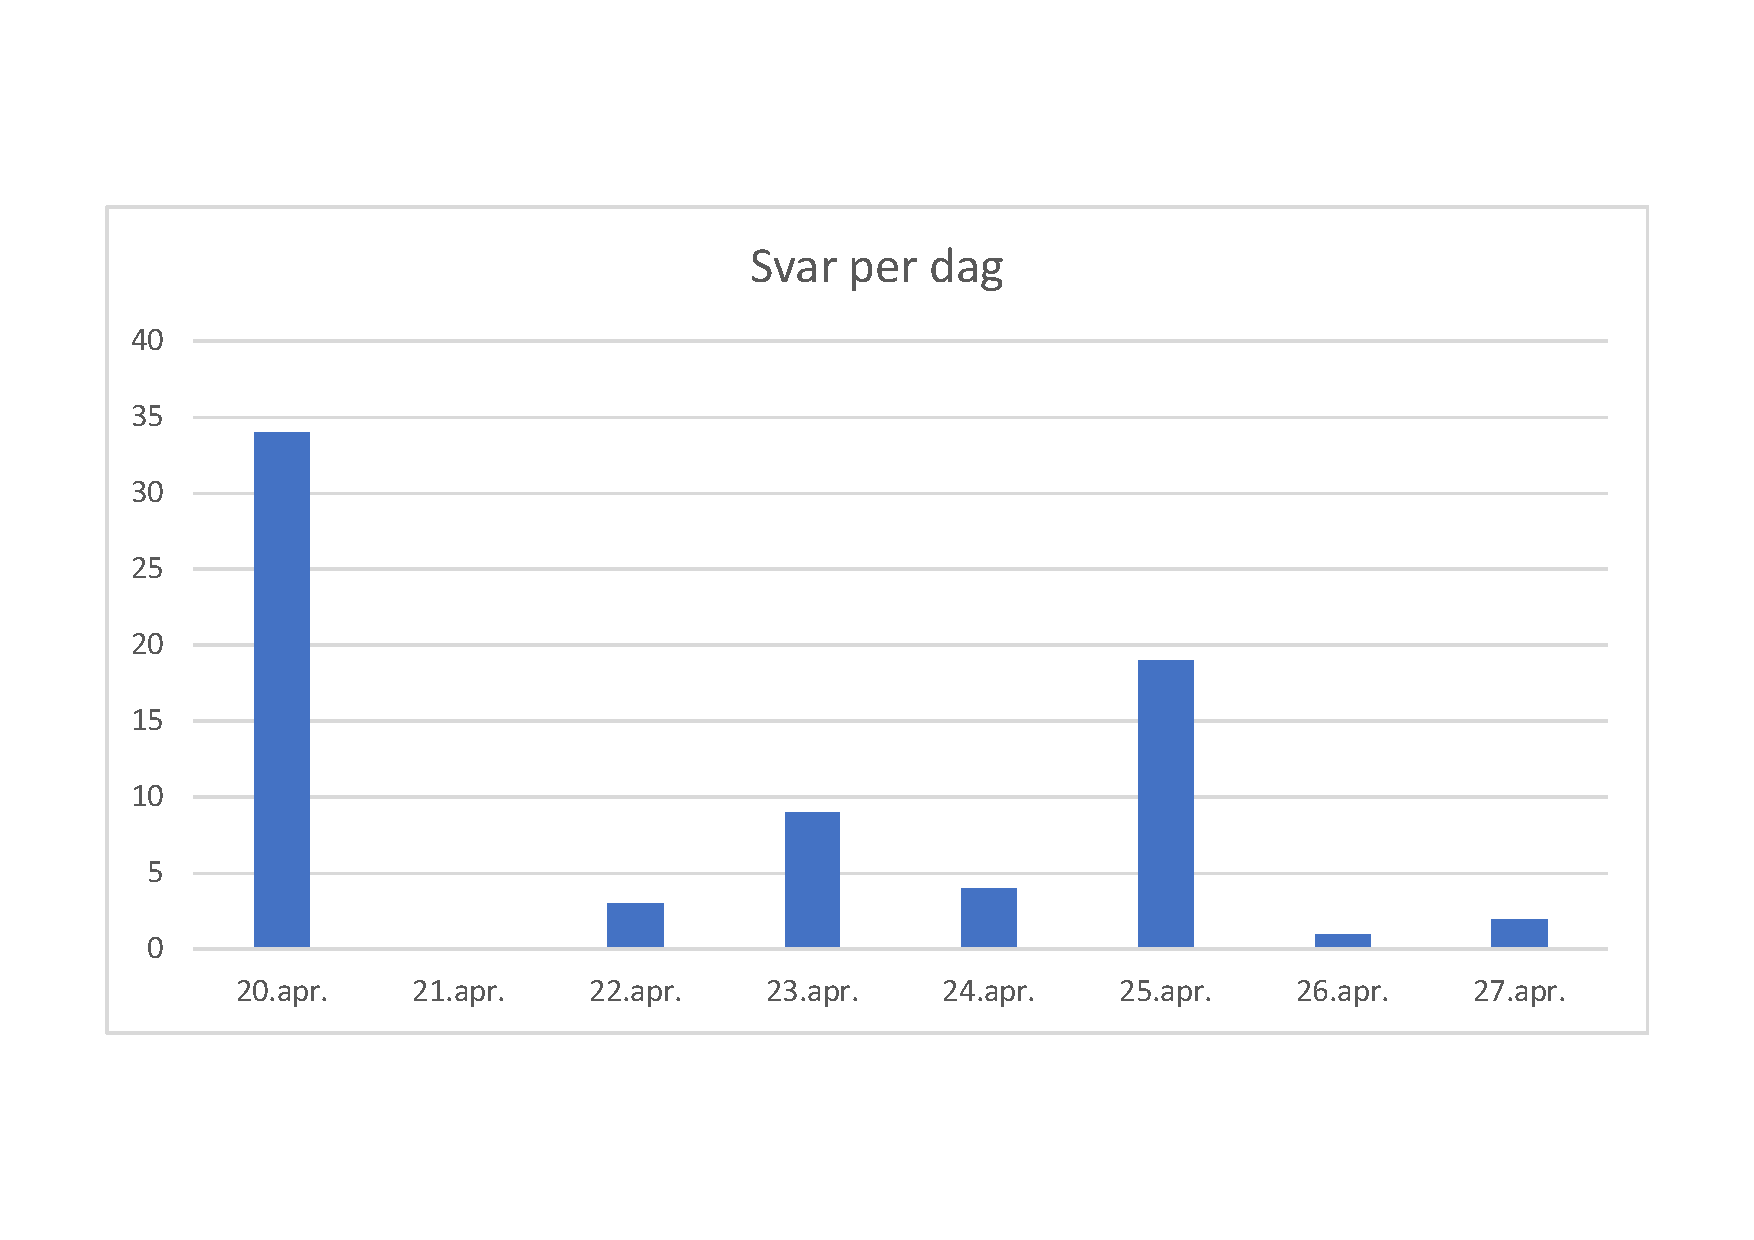
\includegraphics[scale=0.5, clip, trim=1cm 3cm 0cm 3cm]{case_2/bilder/spss/svar_per_dag.pdf}
    \caption[Svar per dag]{Antall svar vi fikk per dag}
    \label{fig:boks}
\end{figure}


%---------------------------------------- DEMOGRAFI ---------------------------------
\section{Demografi}
I denne delen fremlegges resultatene fra demografien i spørreundersøkelsen. Disse blir om mulig sammenliknet med generelle tall fra NTNU for å få et innblikk i demografien til de som har blitt kompromittert, kontra NTNU sine ansatte og studenter generelt. Vi fokuserer stort sett på de ansatte siden antall studenter i undersøkelsen var få.

\subsection{Aldersgruppe}
Aldersgruppene ble kategorisert i intervaller på 10 år. Fra de ulike kategoriene fikk vi:

\begin{itemize}
    \item Under 20: 1 person
    \item 20-29: 3 personer
    \item 30-39: 13 personer
    \item 40-49: 27 personer
    \item 50-59: 11 personer
    \item 60-69: 9 personer
    \item 70 eller over: 8 personer
\end{itemize}

Under ser vi aldersfordelingen visuelt fremstilt i et histogram.

\begin{figure}[H]
    \centering
    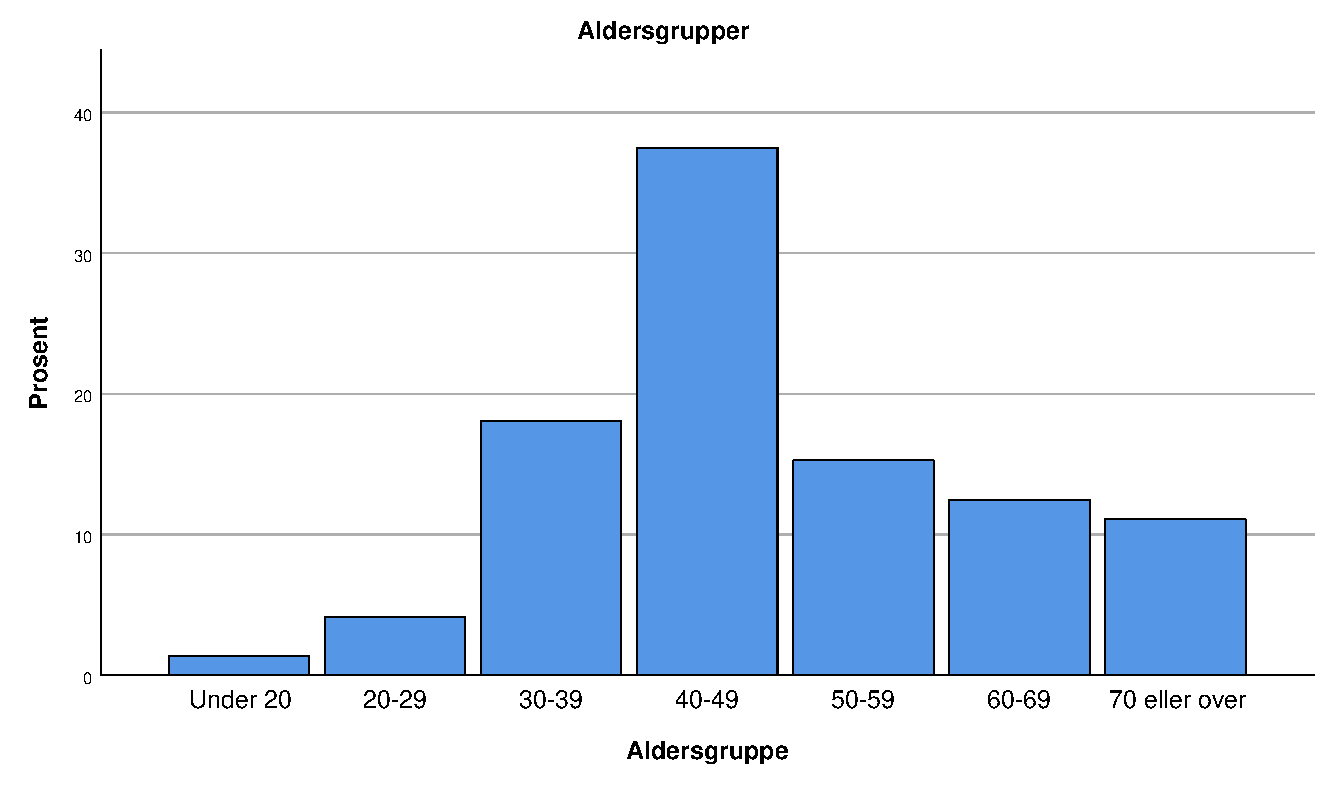
\includegraphics[scale=0.5]{case_2/bilder/spss/aldersgrupper.pdf}
    \label{fig:aldersgruppe}
    \caption[aldersgruppe]{Aldersgrupper av respondentene}
\end{figure}

Ut fra resultatene kan vi konkludere med at de som har blitt kompromittert er stort sett middelaldrene til eldre personer. Disse personene er også noe eldre enn gjennomsnittsalderen til de som jobber ved NTNU \cite{MorkRapport}. 

\subsection{Kjønn}
I spørreundersøkelsen kunne du velge å ikke oppgi kjønn, men dette alternativet var det ingen som benyttet seg av. Av de 72 respondentene var det 45 kvinner og 27 menn. Det er henholdsvis 62,5\% og 37,5\%. Under er kjønnsfordelingen visualisert i et sektordiagram.

\begin{figure}[H]
    \centering
    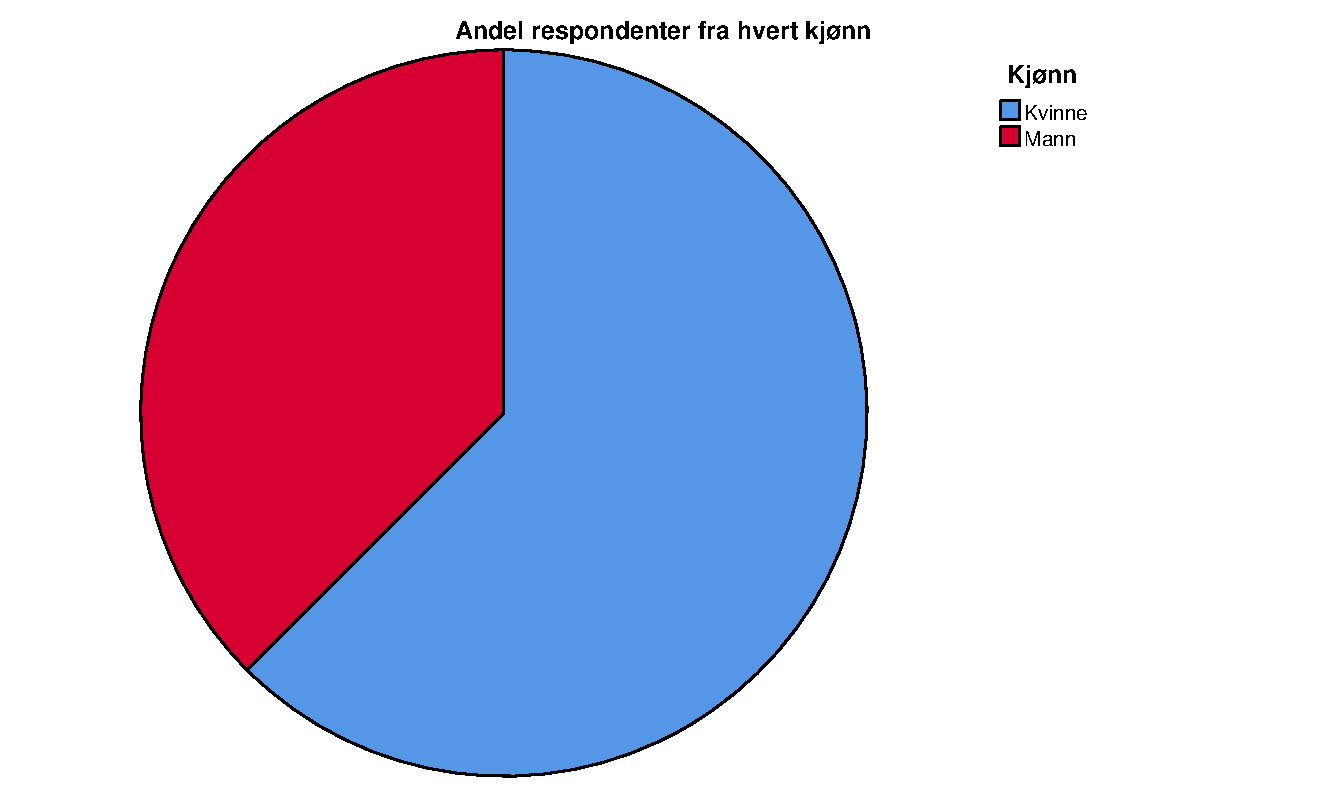
\includegraphics[scale=0.5]{case_2/bilder/spss/kjonn.pdf}
    \label{fig:kjonn}
    \caption[kjonn]{Andel fra hvert kjønn}
\end{figure}

De fleste av de som har svart er kvinner. Av de ansatte ved NTNU er det 41\% kvinner totalt \cite{NTNUfakta}. Totalt sendte vi ut spørreundersøkelsen til 167 e-postadresser, der 157 av de mottok. Vi har tall på at 91 av de 167 vi først sendte ut til var kvinner. Dette er omtrent 55\%. For å kunne si noe om antallet kvinner som svarte på spørreundersøkelsen må vi se på om svarene våre er representative for hele samplet. Vi brukte en kalkulator for å regne ut konfidensintervallet for vårt sample \cite{SSCalc}. Utregningen kom fram til at vi er 95\% sikre på at feilmarginen for dette spørsmålet er \(\pm 8,5\%\). I og med at andelen kvinner totalt på NTNU er 41\%, kan vi fastslå at kvinner er noe mer utsatt for å kontoen kompromittert, men denne forskjellen er ikke stor. 

\subsection{Primærrolle}
Det ble definert to primærroller for å skille mellom ansatte og studenter. Dette ble gjort fordi oppdragsgiver hadde info på at det både var studenter og ansatte som hadde blitt kompromittert. Av de 72 respondentene var det 6 studenter og 66 ansatte. Dette er henholdsvis 8,3\% og 91,7\%. Sektordiagrammet under viser fordelingen. 

\begin{figure}[H]
    \centering
    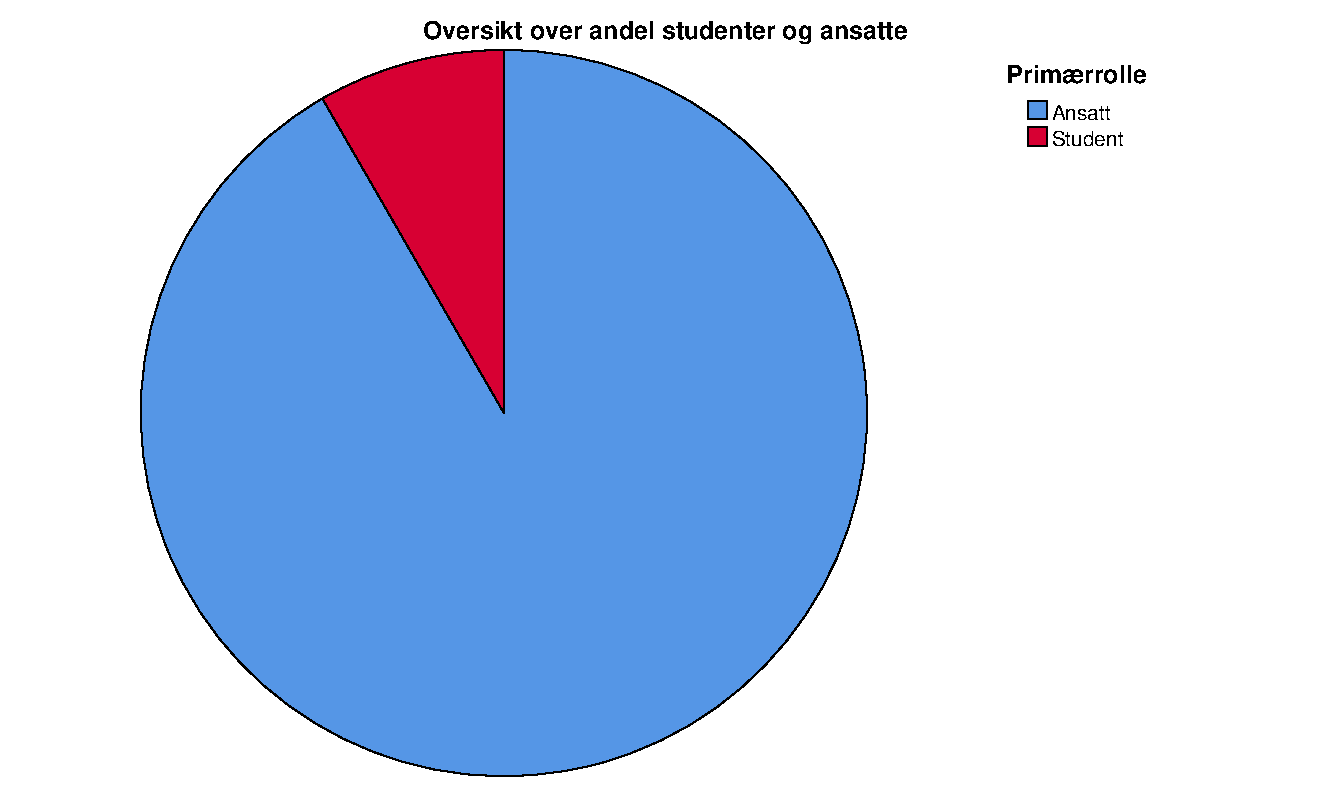
\includegraphics[scale=0.5]{case_2/bilder/spss/primaerrolle.pdf}
    \label{fig:primaerrolle}
    \caption[primaerrolle]{Primærrolle ved NTNU}
\end{figure}

Fra dataene kan vi se at ansatte er overrepresentert i de som blir kompromittert. Vi har data på at det er 18 studenter i vårt sample, altså står studenter for omtrent 10\% av de kompromitterte. På samme måte som i forrige seksjon, ble konfidensintervallet regnet ut \cite{SSCalc}. Utregningen kom frem til at vi er 95\% sikre på at feilmarginen er på \(\pm 5,12\%\). Derfor kan vi med rimelig sikkerhet si at trusselaktørenes målgruppe er de ansatte og ikke studenter. 

\subsection{Primærby}
Av de 72 respondentene var det bare en fra Ålesund og resten var fra Trondheim. Det var ingen respondenter fra Gjøvik. 

\subsection{År ved NTNU}
Bare 6 personer, eller 8,3\% av respondentene hadde jobbet eller studert ved NTNU i under 2 år og i 2 til 4 år. 9 personer, eller 12,5\% hadde jobbet eller studert her i 5 til 9 år, og 15 personer, eller 20,8\% hadde jobbet eller studert her i 10 til 15 år. Hele 36 personer, eller akkurat halvparten av respondentene har vært hos NTNU i over 15 år. En oversikt over disse tallene finnes i histogrammet under. 

\begin{figure}[H]
    \centering
    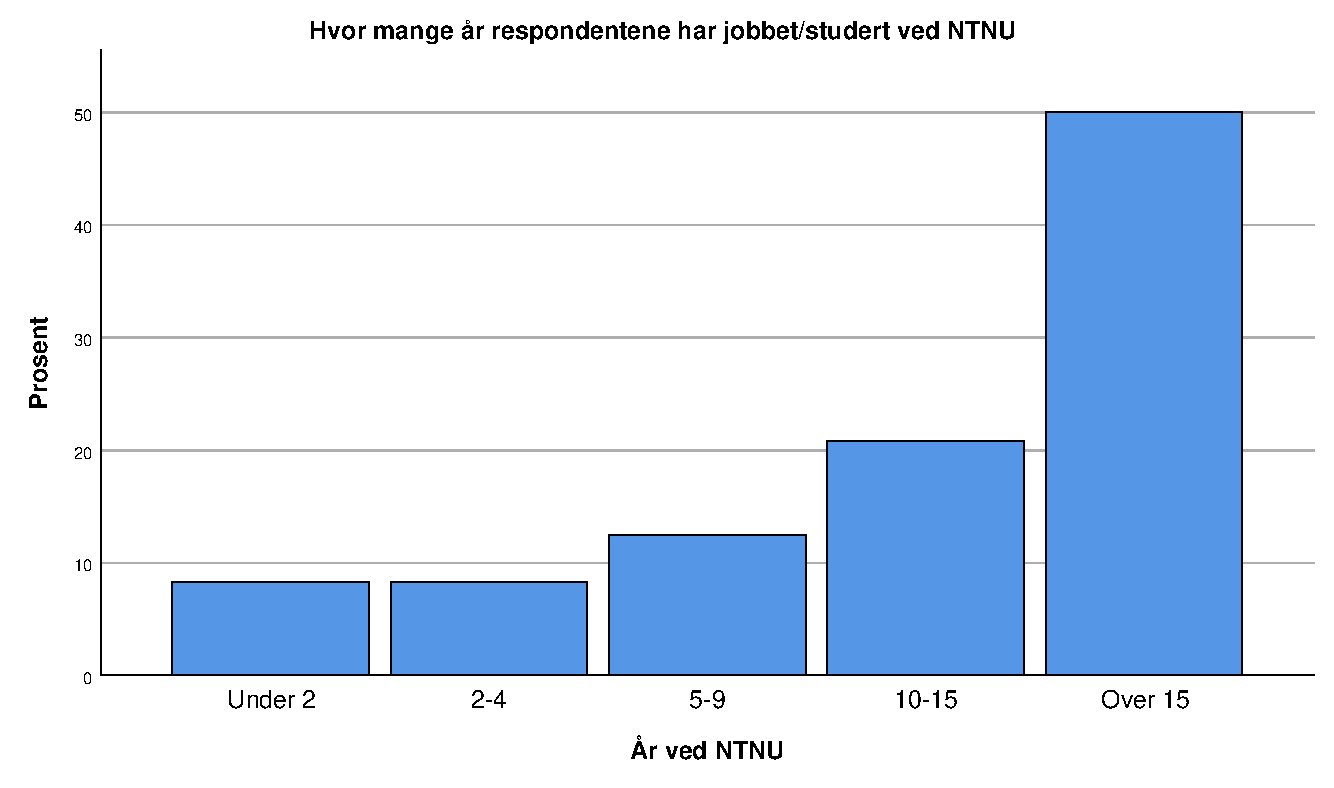
\includegraphics[scale=0.5]{case_2/bilder/spss/aarvedNTNU.pdf}
    \label{fig:aarvedNTNU}
    \caption[aarvedNTNU]{Antall år ved NTNU}
\end{figure}


\subsection{Konklusjon}

%---------------------------------------BEVISSTHET PÅ SIKKERHET---------------------------------
\section{Bevissthet på sikkerhet}
Spørsmålene skulle gi svar på hvor sikkerhetsbevisst en tenker når man besøker nettsider, lager passord og sjekker e-post. Hypotesen som ble fremhevet her var at folk generelt sett er lite bevisste. 

Histogrammet i figur \ref{fig:bevisst-nettsider} viser en tilnærmet normalfordelt situasjon, men med noe fler svar på høyresiden. De fleste er derfor litt mer bevisste på sikkerhet når de besøker nettsider enn de er ubevisste. 
\begin{figure}[H]
    \centering
    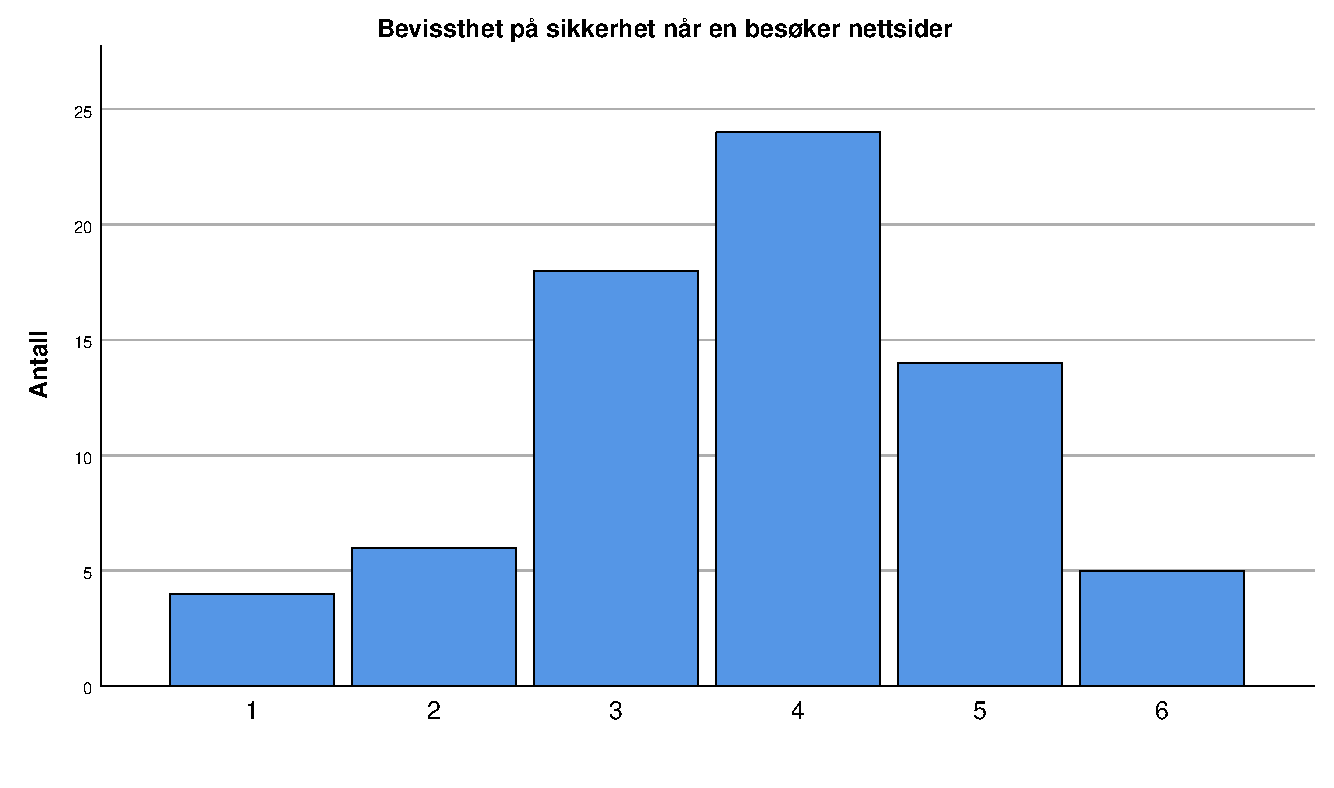
\includegraphics[scale=0.5]{case_2/bilder/spss/bevisst_nettsider.pdf}
    \caption[bevisst-nettsider]{Bevissthet på sikkerhet når en besøker nettsider}
    \label{fig:bevisst-nettsider}
\end{figure}

Når det kommer til sikkerhet når en lager passord svarer respondentene at de generelt sett er bevisste på dette. Figur \ref{fig:bevisst-passord} under viser at fordelingen er konsentrert hovedsaklig på høyresiden.
\begin{figure}[H]
    \centering
    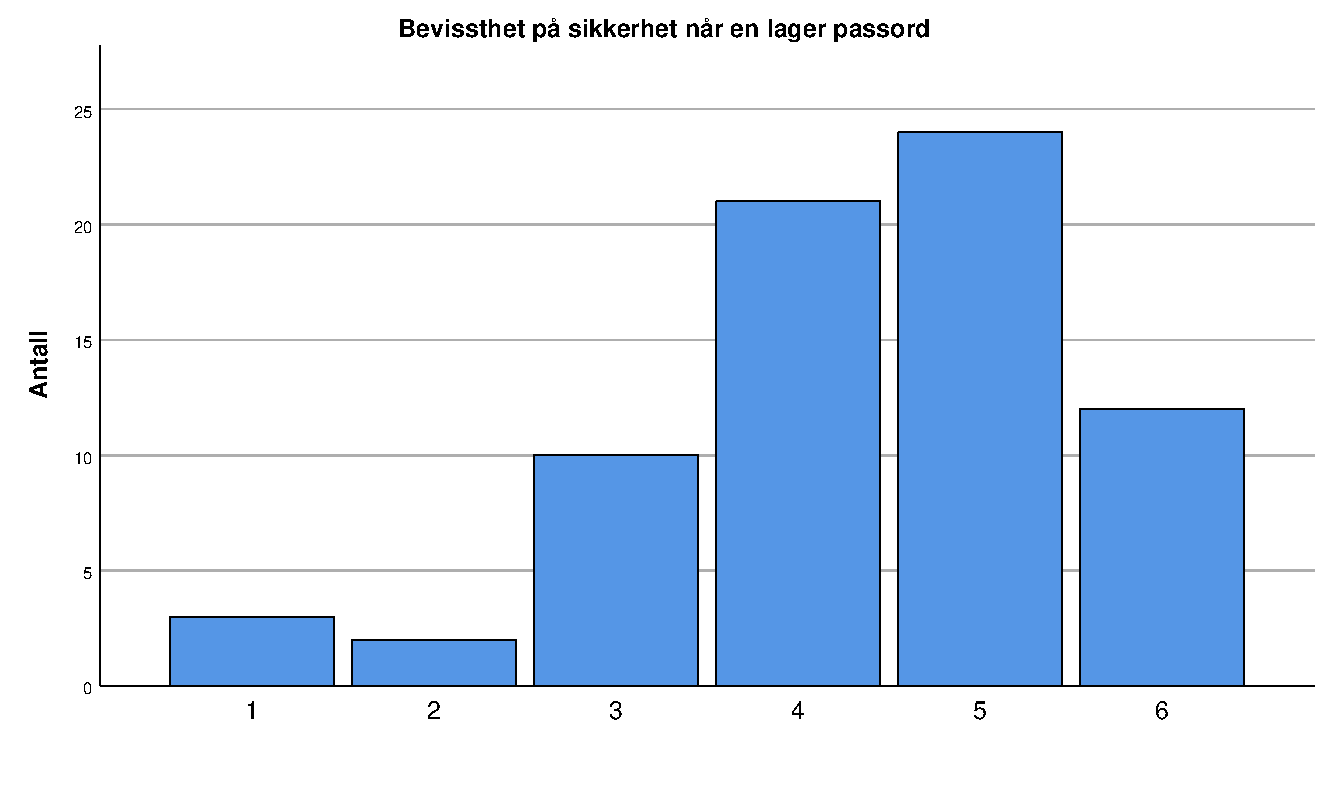
\includegraphics[scale=0.5]{case_2/bilder/spss/bevisst_passord.pdf}
    \caption[bevisst-passord]{Bevissthet på sikkerhet når en lager passord}
    \label{fig:bevisst-passord}
\end{figure}

Figur \ref{fig:bevisst-e-post} under viser bevissthetsfordelingen når det kommer til sjekking av e-post. Dette var noe vi spesielt ønsket å se på siden en av hovedhypotesene våre til kompromitterte brukerkontoer er phishing. Histogrammet viser at respondentene stort sett er bevisste på sikkerhet når de sjekker e-post.
\begin{figure}[H]
    \centering
    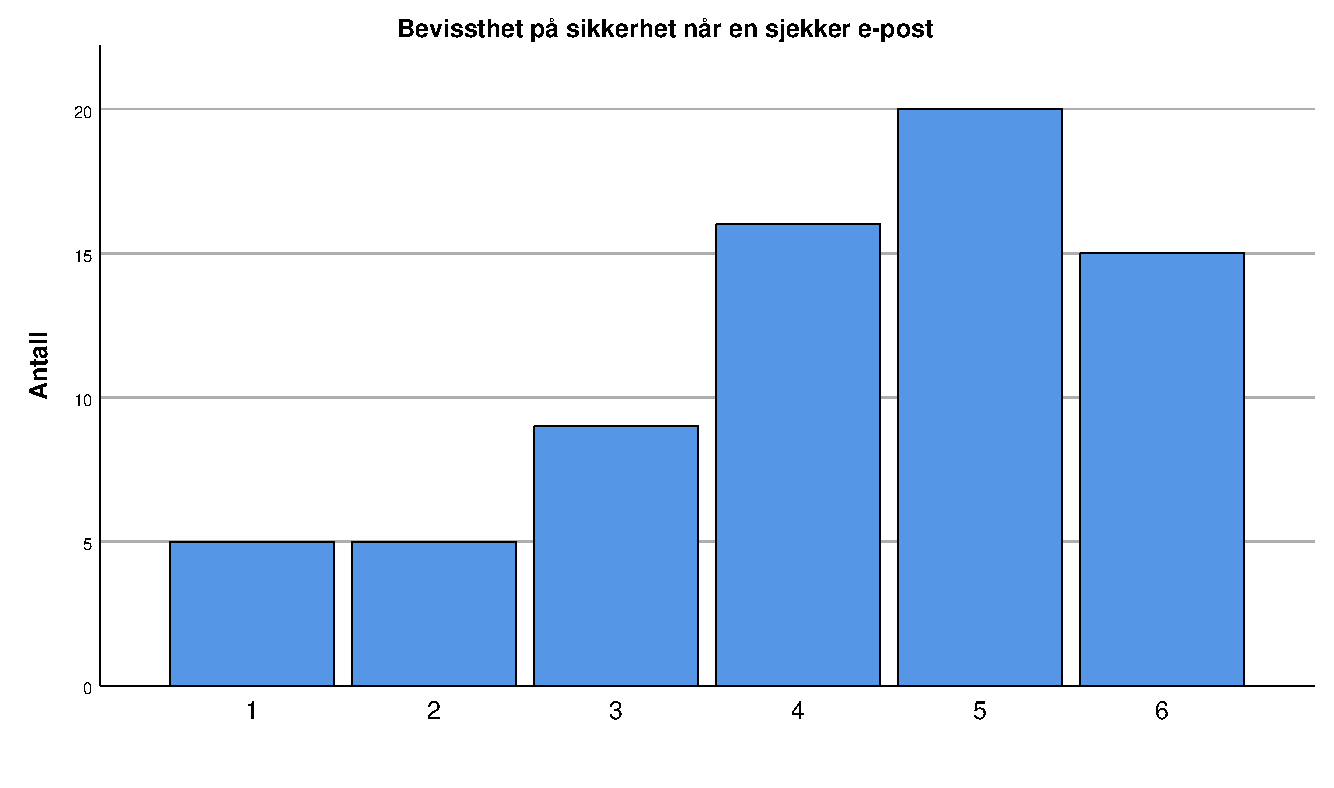
\includegraphics[scale=0.5]{case_2/bilder/spss/bevisst_e-post.pdf}
    \caption[bevisst-e-post]{Bevissthet på sikkerhet når en sjekker e-post}
    \label{fig:bevisst-e-post}
\end{figure}

\subsection{Konklusjon}
Det viser seg at hypotesen vår ikke stemte helt. Vi tror derimot at denne bevisstheten ikke er nok, eller til og med mangelfull. Vi har grunn til å tro at respondentene overvurderer sin egen bevissthet og kompetanse, basert på resten av svarene i denne spørreundersøkelsen. I etterkant har det blitt reist spørsmål rundt validiteten til disse spørsmålene, fordi det spørres om hvor bevisste de er nå, og ikke før de ble kompromittert. Enkelte har gitt tilbakemelding om at de har endret sine rutiner og blitt mer bevisst på sikkerhet i etterkant. Derfor er det grunn til å mene at vi burde spesifisert i spørsmålene hvor bevisste de var før de ble kompromittert.
%---------------------------------------KJENNSKAP RETNINGSLINJER REGLEMENT OG PRINSIPPER---------------------------------
\section{Kjennskap til retningslinjer, reglementer og prinsipper}
Disse spørsmålene handler om hvor godt kjennskap respondentene har til NTNU sine retningslinjer for behandling av autentiseringsdata, IT reglementet og prinsipper for informasjonssikkerhet. Hypotesen vi hadde her var at de aller fleste hadde lite kjennskap til disse.

Det viser seg fra figur \ref{fig:retningslinjer} at respondentene kan lite om NTNU sine retningslinjer for behandling av brukernavn, passord og andre autentiseringsdata. 
\begin{figure}[H]
    \centering
    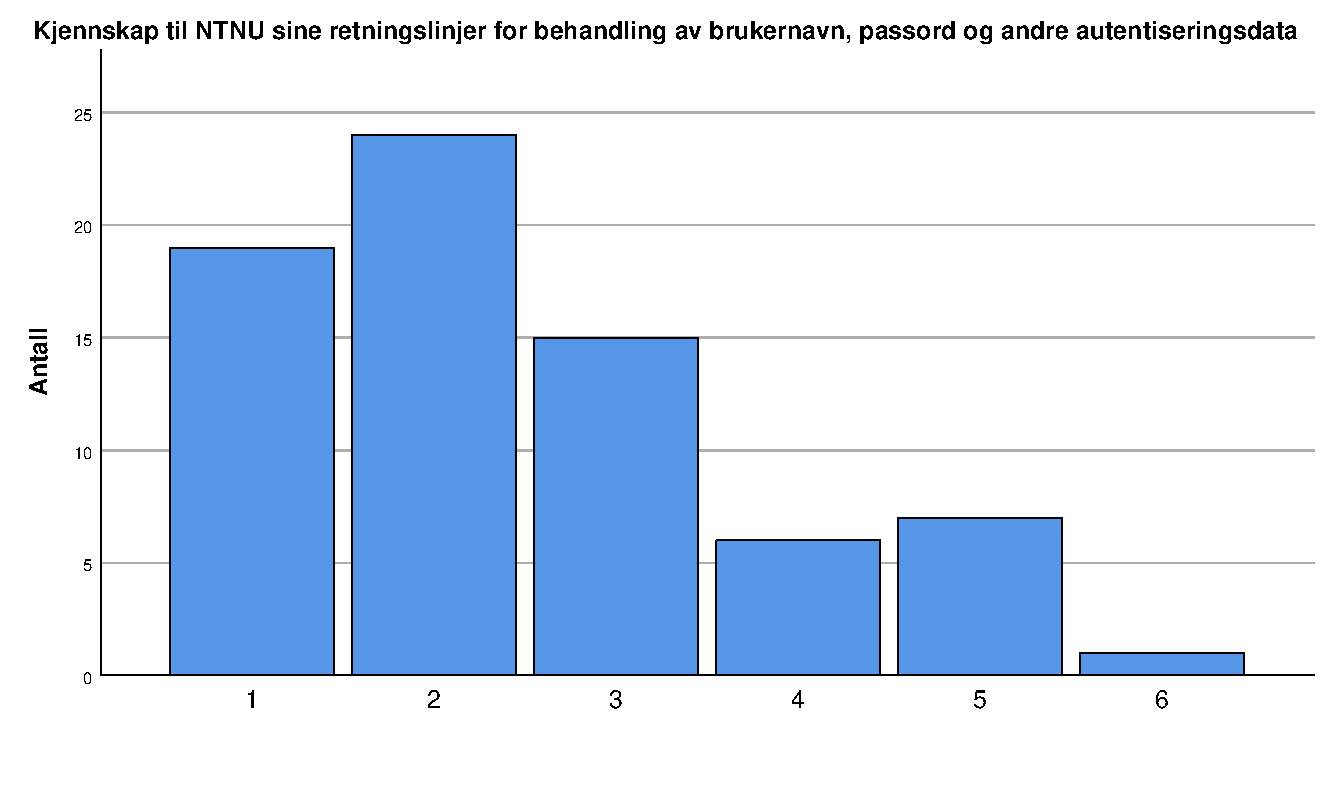
\includegraphics[scale=0.5]{case_2/bilder/spss/retningslinjer.pdf}
    \caption[retningslinjer]{Kjennskap til retningslinjer}
    \label{fig:retningslinjer}
\end{figure}

Figur \ref{fig:ITreglement} viser at respondentene ikke kjenner så godt til IT reglementet til NTNU. Over 70\% svarte tre eller under på hvor godt de kjente IT reglementet til NTNU, der 1 var lite kjent og 6 var meget kjent.  
\begin{figure}[H]
    \centering
    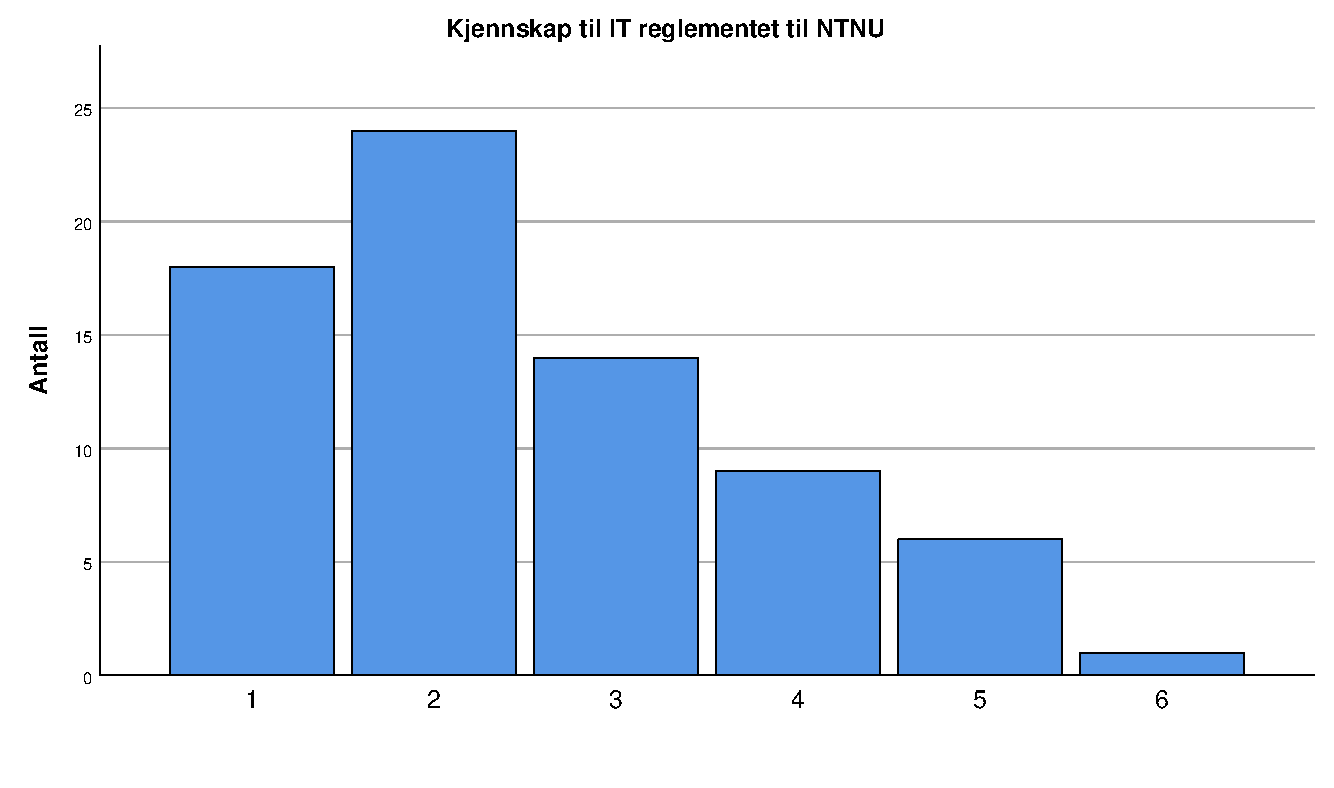
\includegraphics[scale=0.5]{case_2/bilder/spss/ITreglement.pdf}
    \label{fig:ITreglement}
    \caption[ITreglement]{Kjennskap til IT reglement}
\end{figure}

Under viser figur \ref{fig:InfoSecPolicy} at folk har dårlig kjennskap til NTNU sine prinsipper for informasjonssikkerhet. Der står det blant annet at brukere er ansvarlige for enhver bruk av innloggingskredentialier og at de holder dette konfidensielt \cite{PrinsInfoSec}. 
\begin{figure}[H]
    \centering
    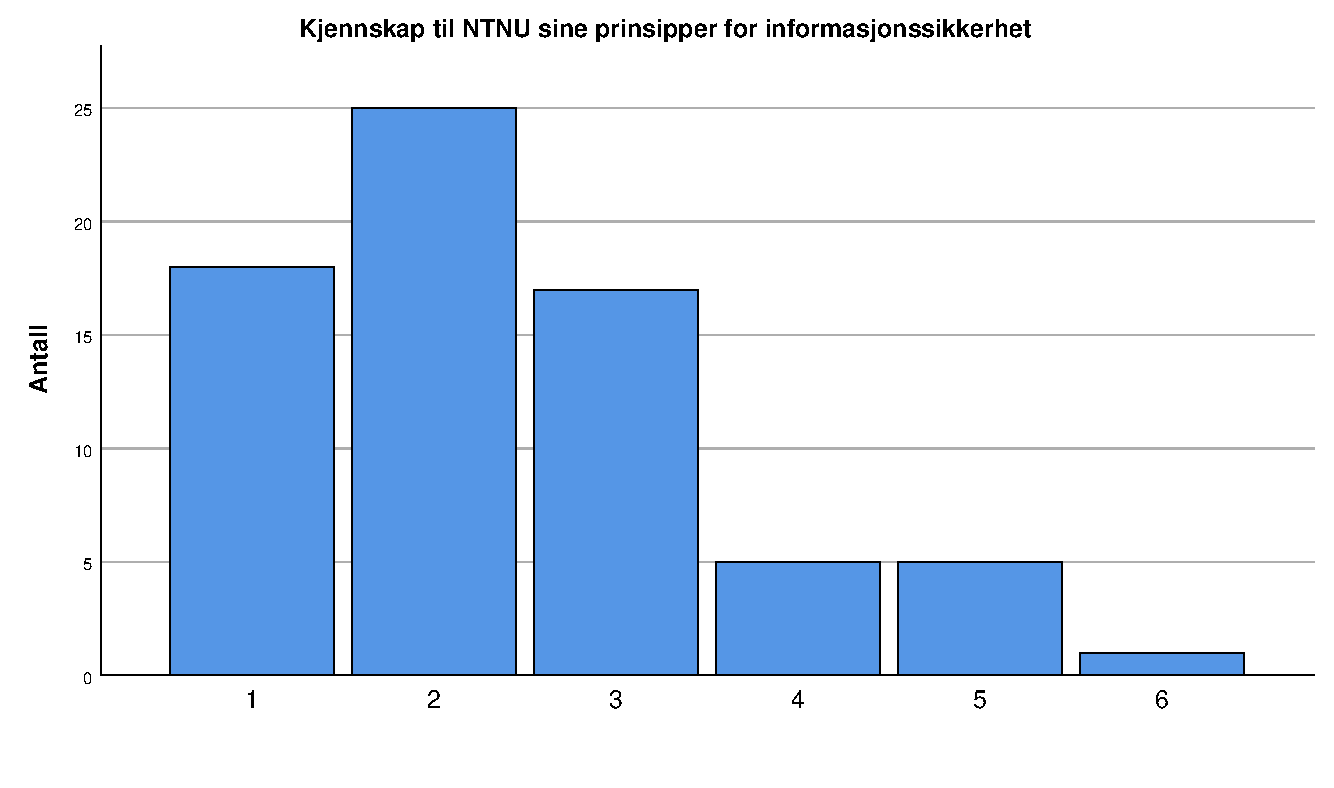
\includegraphics[scale=0.5]{case_2/bilder/spss/InfoSecPolicy.pdf}
    \caption[InfoSecPolicy]{Kjennskap til NTNU sine prinsipper for informasjonssikkerhet}
    \label{fig:InfoSecPolicy}
\end{figure}

Det viser seg at hypotesen vi hadde stemte. Det er lite kjennskap til dokumentasjon på informasjonssikkerhet. Dersom disse dokumentene skal være noe mer enn hyllevarmere må det komme bedre informasjon.


%---------------------------------------Oversikt---------------------------------
\section{Respondentenes egen oversikt}
Her så var vi interessert i å finne ut om når de fant ut at kontoen var blitt kompromittert. Det viser seg at det ikke stemte. Over 60\% av respondentene viste ikke at kontoen var blitt kompromittert før Seksjon for Digital Sikkerhet ringte, og kun 20\% svarte at de fant ut av det før og resten svarte at de ikke vet.
\begin{figure}[H]
    \centering
    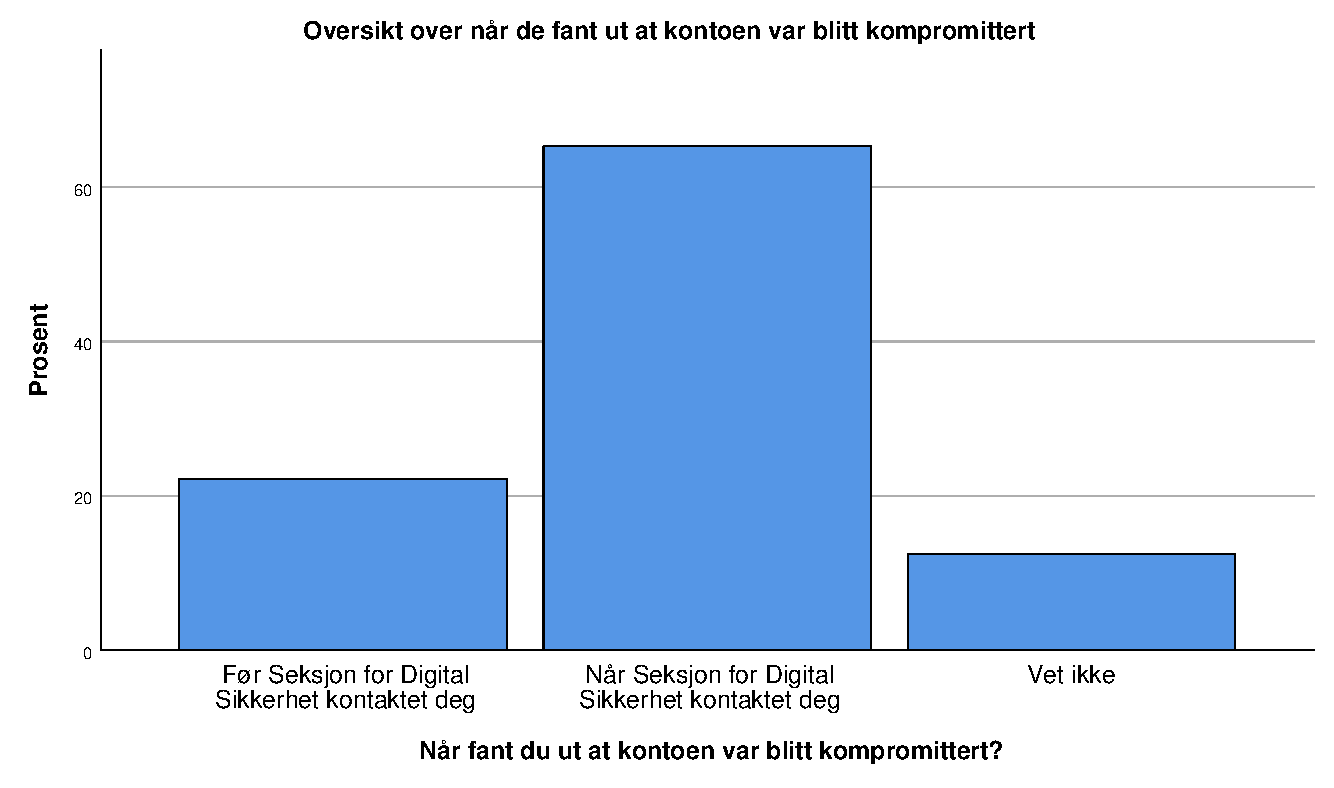
\includegraphics[scale=0.5]{case_2/bilder/spss/Fant_ut_kompromittert.pdf}
    \caption[fant-ut-kompromittert]{Viser når de fant ut at de var blitt kompromittert}
    \label{fig:fant-ut-kompromittert}
\end{figure}
Hypotesen vår her var korrekt. De vet ikke at de har blitt kompromittert før de blir kontaktet.


Respondentene svarte at de trodde kontoen var kompromittert mindre enn tre måneder før Seksjon for Digital Sikkerhet kontaktet dem. Denne statistikken kan vi ikke være helt sikre på, fordi halvveis i undersøkelsen fikk vi tilbakemeldiner på at det var flere som ikke ville fullføre spørreundersøkelsen siden dette svaret var obligatorisk og det ikke var noe alternativ for ``vet ikke''. Vi fjernet da kravet om å svare halvveis ut i undersøkelsen. 
\begin{figure}[H]
    \centering
    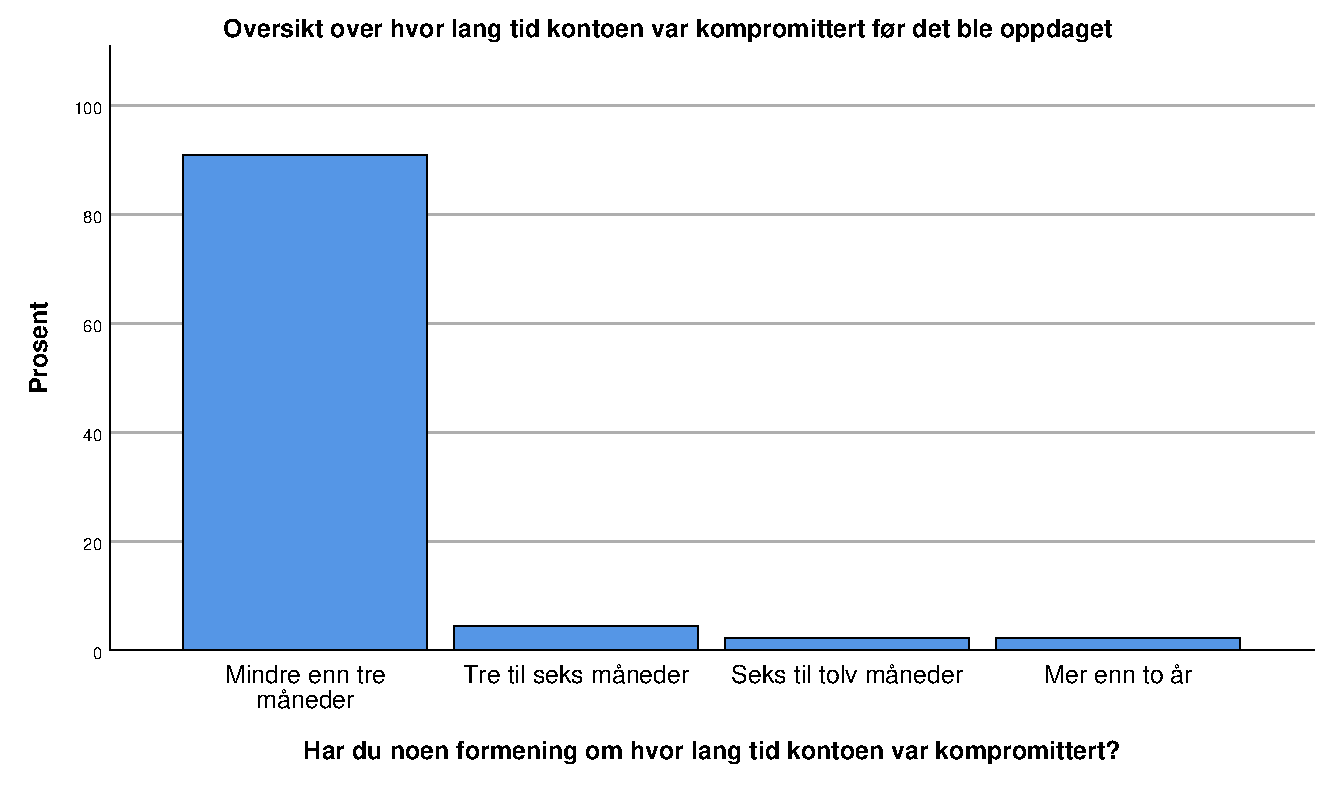
\includegraphics[scale=0.5]{case_2/bilder/spss/lang_tid_konto_kompromittert.pdf}
    \caption[fant-ut-kompromittert]{Viser når de fant ut at de var blitt kompromittert}
    \label{fig:fant-ut-kompromittert}
\end{figure}

\subsection{Formening om hvordan det skjedde}
Dette spørsmålene handlet om respondentene hadde noen formening om hvordan kontoen ble kompromittert. Affinitetsdiagramet viser at respondentene i hovedsak ikke har noen formening om hvordan kontoen ble kompromittert. Over 85\% svarte at de ikke hadde noen formening om hvordan kontoen ble kompromittert. MULIG FOR FEILTOLKING AV SVAR
\begin{figure}[H]
    \centering
    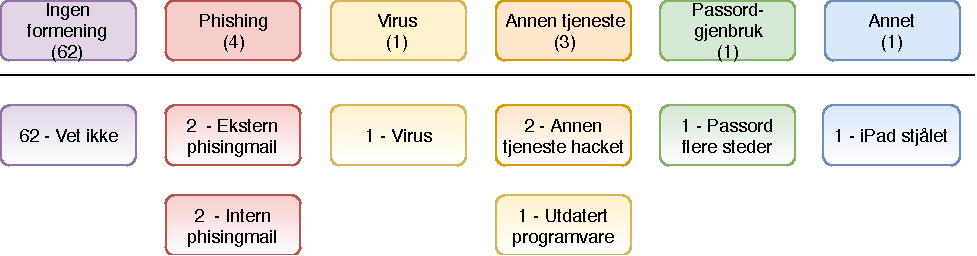
\includegraphics[scale=0.8]{case_2/bilder/Affinitetsdiagram.pdf}
    \caption[affinitetsdiagram]{Affinitetsdiagram av respondentenes formening over hvordan kontoen ble kompromittert}
    \label{fig:case2-affinitetsdiagram}
\end{figure}

\subsection{Konklusjon}
Ut fra svarene kan en konkludere med at de som får kontoen kompromittert i hovedsak ikke vet at den har blitt kompromittert eller når den ble kompromittert. De vet heller stort sett ikke hvordan det har skjedd. 

%---------------------------------------BRUKER- OG PASSORDVANER---------------------------------
\section{Bruker- og passordvaner}
Som vi kan se i figur \ref{fig:epost-jobb} under, bruker over 60\% av respondentene NTNU e-posten til å registrere seg på tjenester i forbindelse med jobb.
\begin{figure}[H]
    \centering
    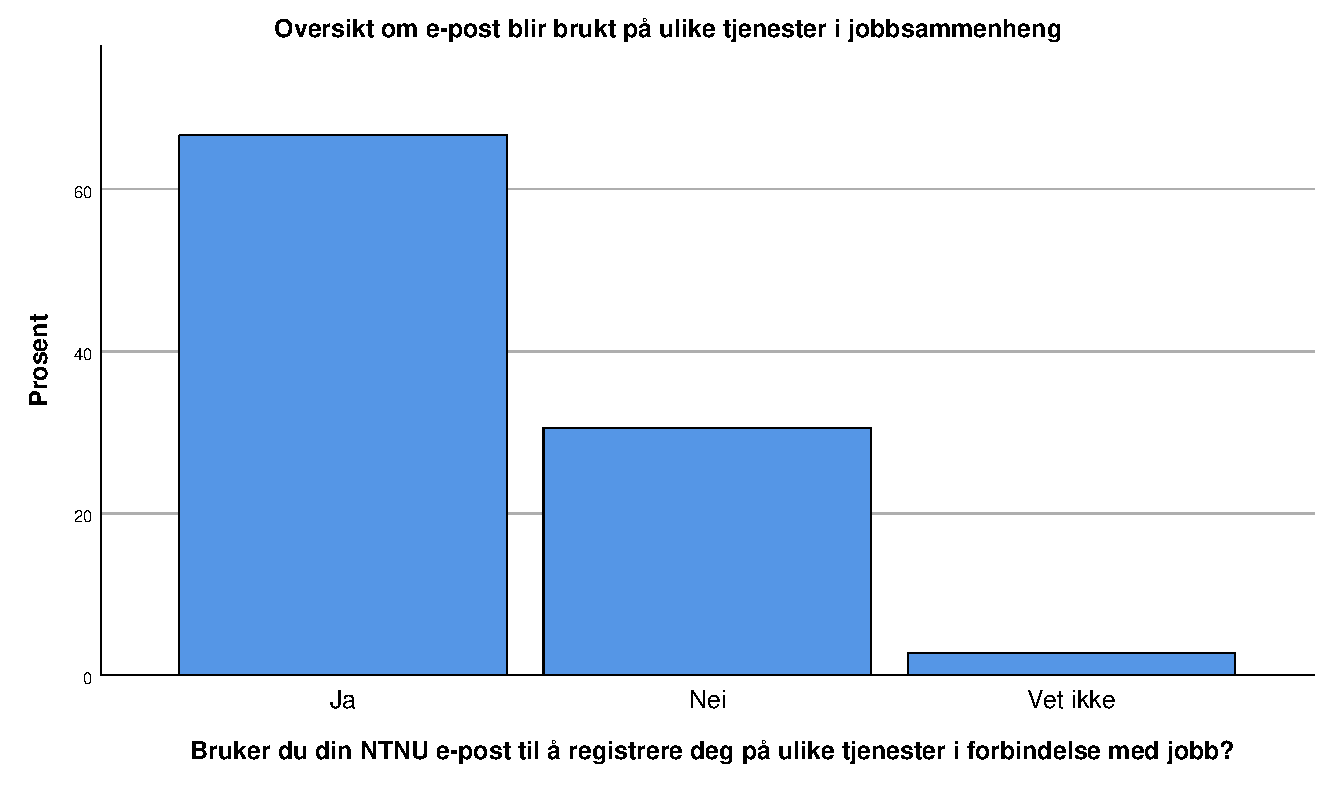
\includegraphics[scale=0.5]{case_2/bilder/spss/epost_jobb.pdf}
    \caption[epost-jobb]{Viser hvor mange som bruker NTNU e-post til andre jobbrelaterte tjenester}
    \label{fig:epost-jobb}
\end{figure}
Hypotesen vår stemte. Over halvparten bruker NTNU e-posten til å registrere seg på tjenester i forbindelse med jobb. 

48,6\% av respondentene bruker NTNU e-posten sin til private tjenester. Den samme andelen gjør ikke det og de restende (2,8\%) har svart at de ikke vet. Dette blir vist i figur \ref{fig:epost-privat}.
\begin{figure}[H]
    \centering
    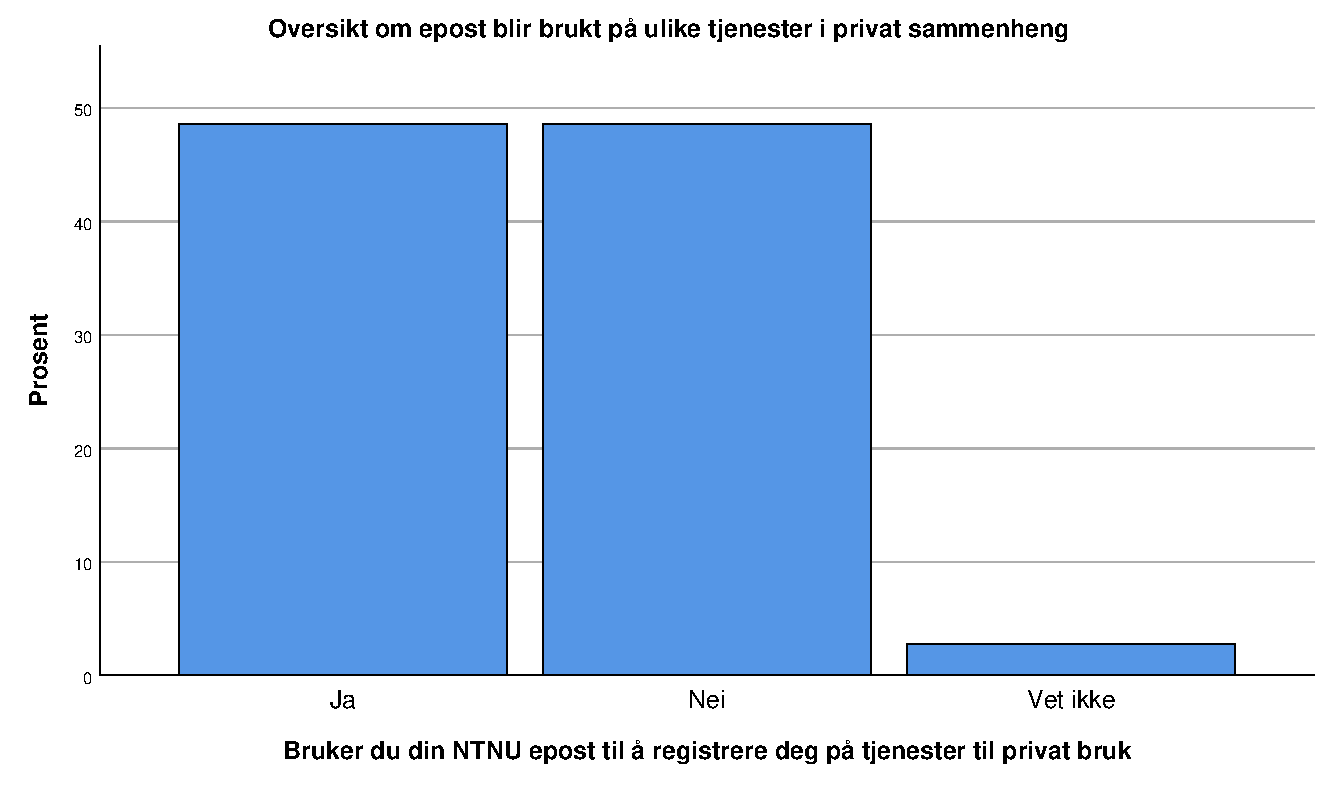
\includegraphics[scale=0.5]{case_2/bilder/spss/epost_privat.pdf}
    \caption[epost-privat]{Viser hvor mange som bruker NTNU e-post til private tjenester}
    \label{fig:epost-privat}
\end{figure}
Hypotesen vår var korrekt, under halvparten bruker NTNU e-posten sin til private tjenester. 

Over 50\% av respondentene bruker NTNU passordet på flere tjenester. Dette vises i figuren under. 
\begin{figure}[H]
    \centering
    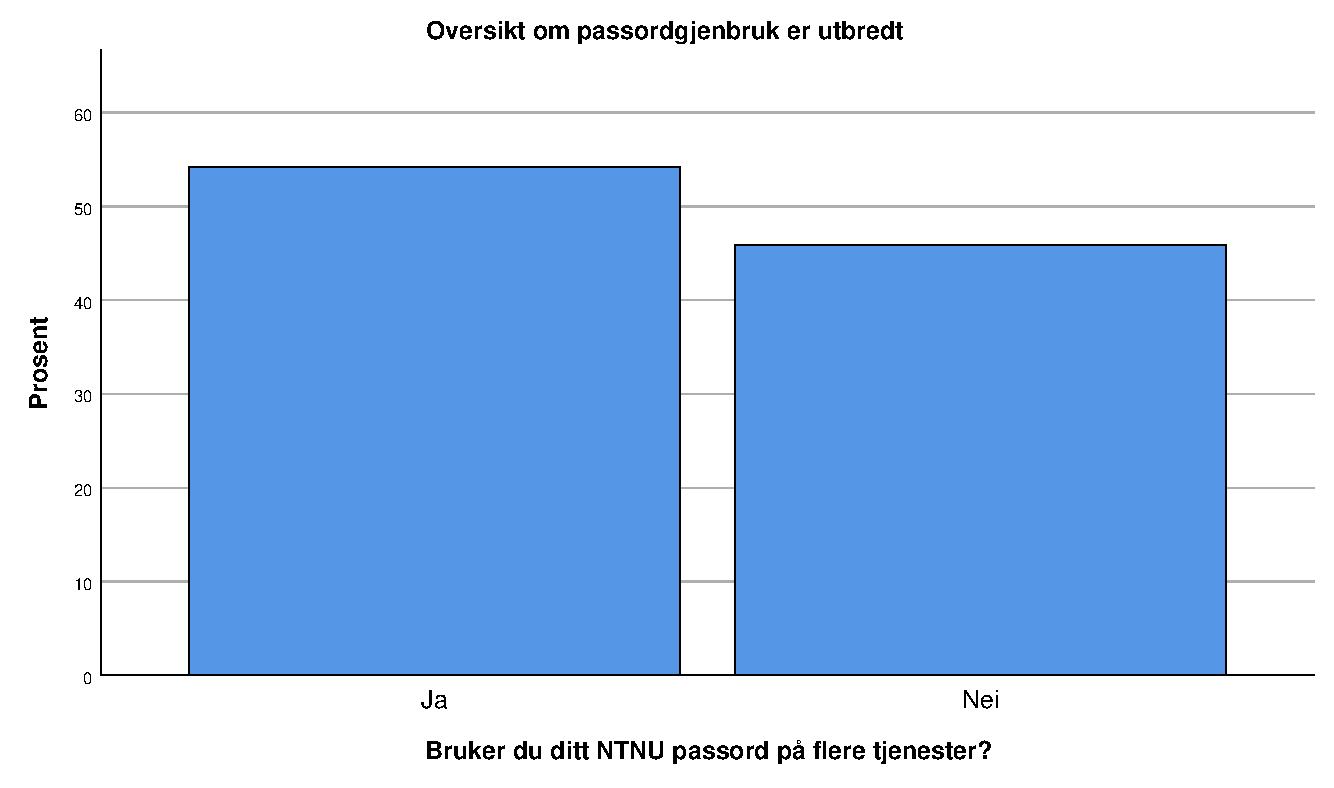
\includegraphics[scale=0.5]{case_2/bilder/spss/passordgjenbruk.pdf}
    \caption[passordgjenbruk]{Oversikt over gjenbruk av NTNU passord}
    \label{fig:passordgjenbruk}
\end{figure}
Hypotesen vår var her korrekt, passordgjenbruk er utbredt på NTNU. 

Over 80\% av respondentene svarte at de ikke brukte regler til å generere passord. Det er mulig for feiltolkning av spørsmålet, i og med at regler kan bety to forskjellige ting. Det kan bety regle, i form av ``Lisa-gikk-til-NTNU'' for NTNU-passord, eller så kan man tolke det som en regel. 
\begin{figure}[H]
    \centering
    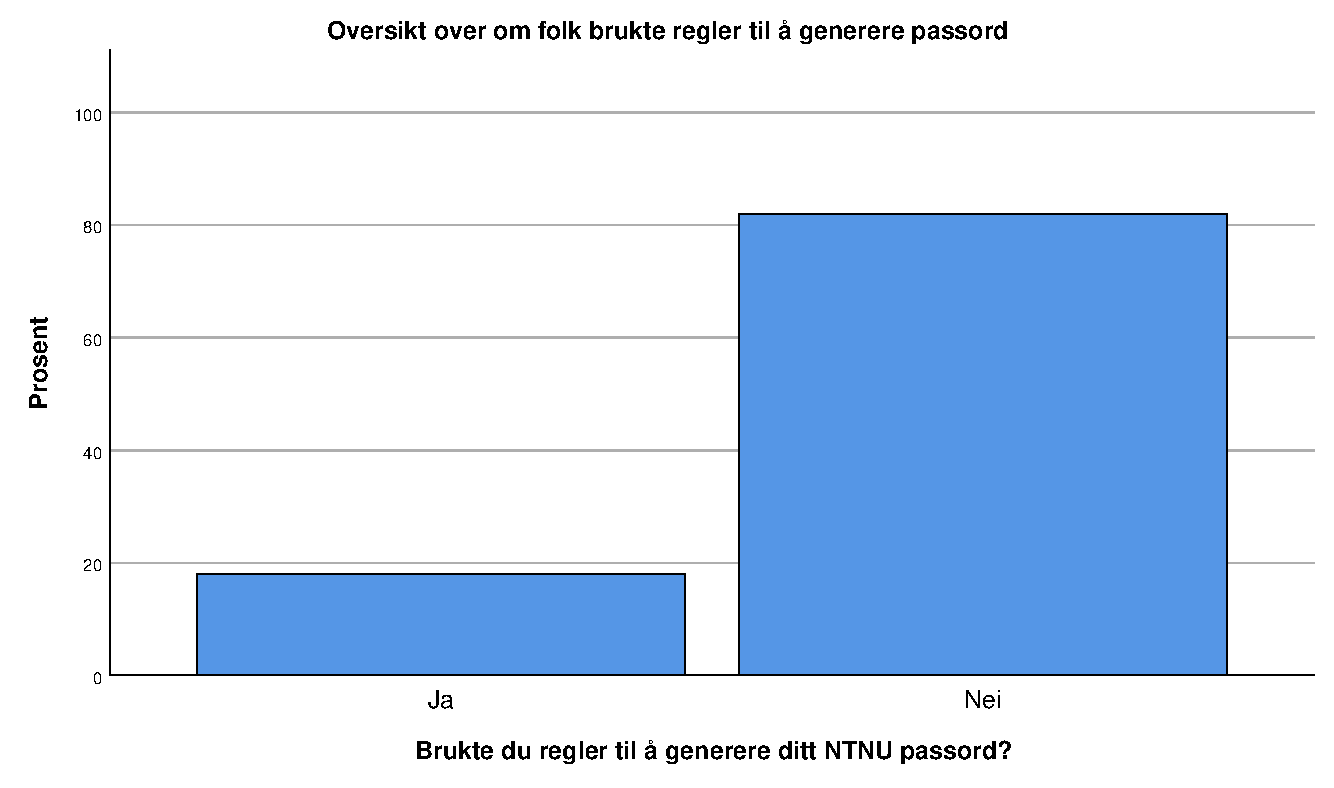
\includegraphics[scale=0.5]{case_2/bilder/spss/regler_passord.pdf}
    \caption[passordregler]{Viser hvor mange som bruker passordregler}
    \label{fig:passordregler}
\end{figure}
Vi kan derfor ikke si om hypotesen vår ble bekreftet eller avkreftet.

Over 80\% av respondentene har passord som er mellom 8-11 tegn. Resterende fordelte seg likt utover de andre valgene. 
\begin{figure}[H]
    \centering
    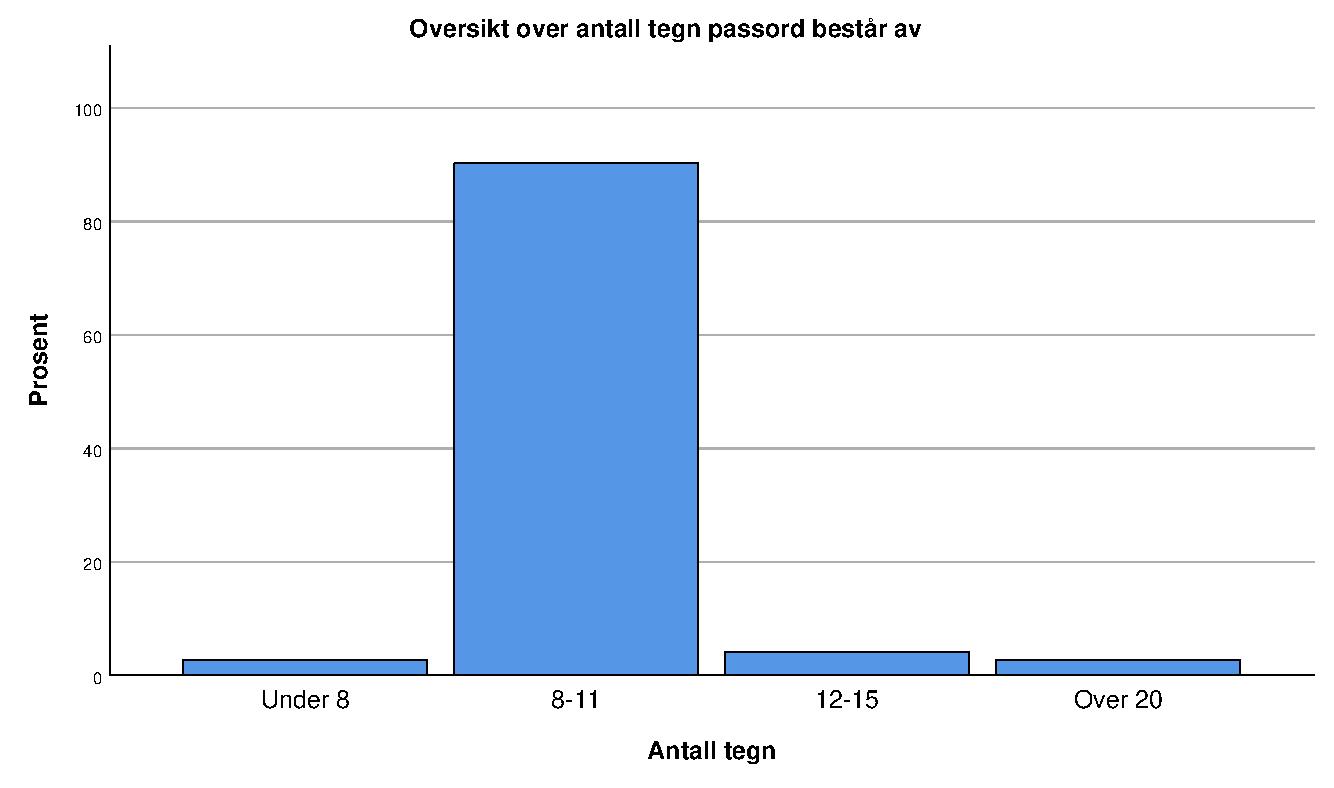
\includegraphics[scale=0.5]{case_2/bilder/spss/antall_tegn.pdf}
    \caption[antalltegn]{Antall tegn på passord}
    \label{fig:antalltegn}
\end{figure}
Hypotesen vår var korrekt, de fleste bruker passord som er under 12 tegn. !!!Burde splitte opp 8-11!!!

Figur \ref{fig:bytter-passord} viser statistikken over hvor ofte respondentene bytter passord. Over 50\% sier at de bytter passord sjeldnere enn hvert andre år, over 20\% sier at de bytter hvert andre år, rett under 20\% sier at de bytter hvert år og resten sier at de bytter hver sjette måned. 
\begin{figure}[H]
    \centering
    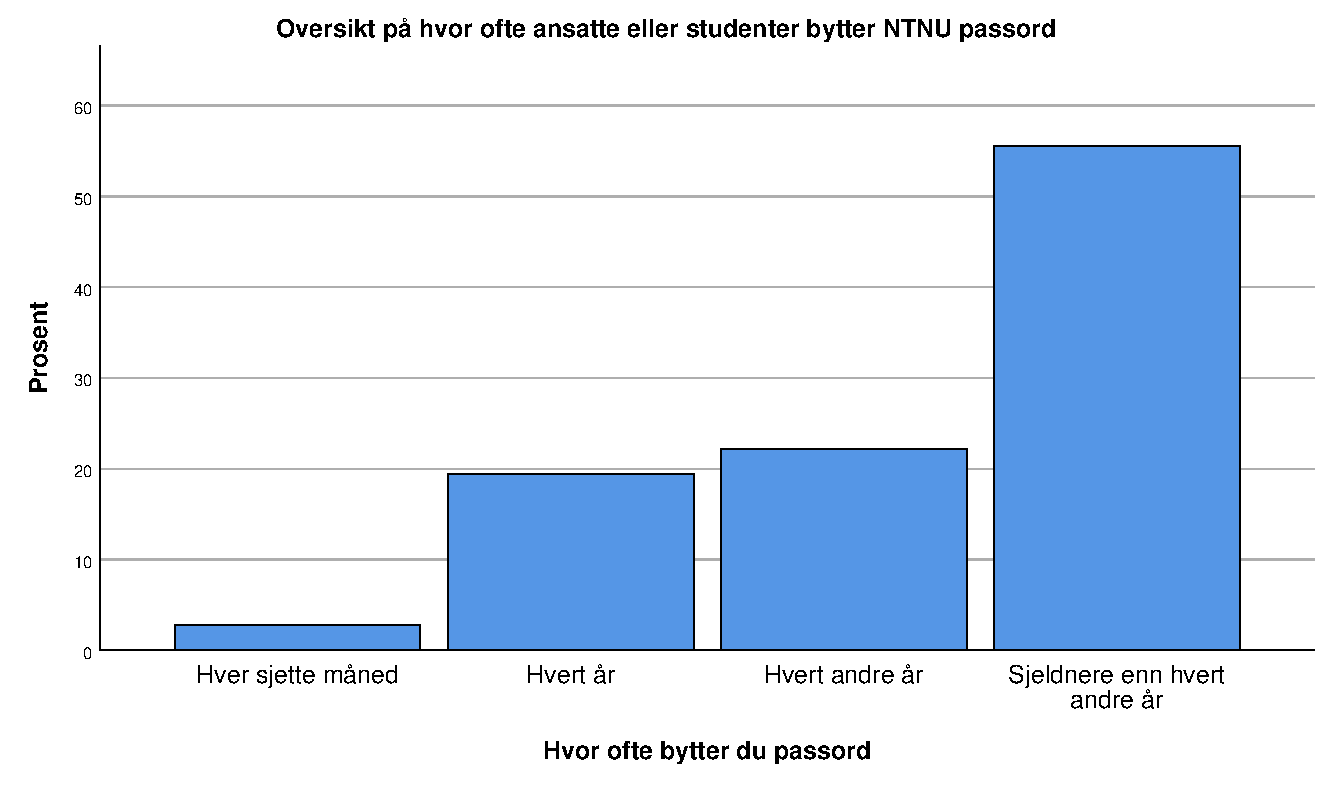
\includegraphics[scale=0.5]{case_2/bilder/spss/bytter_passord.pdf}
    \caption[bytter-passord]{Viser hvor ofte de bytter passord}
    \label{fig:bytter-passord}
\end{figure}
Hypotesen var korrekt, flertallet av respondentene bytter passord sjeldnere enn hvert andre år. I henhold til IT-reglementet over passord, brukernavn og authentiseringsdata så skal passord byttes hver sjette måned og tvungen passordbytte hvert år. Dette viser at respondentene ikke kjent med IT-reglementet og reglementet blir ikke overholdt.

Her så ser vi antallet som sier at de har fått opplæring i passordsikkerhet fra NTNU. Ut fra tabellen ser vi at under 80\% av respondentene sier at de ikke har fått opplæring i passordsikkerhet. 15\% sier at de ikke vet om de har fått opplæring og resten sier at de har fått det. Figur \ref{fig:passordsikkerhet} viser dette. 
\begin{figure}[H]
    \centering
    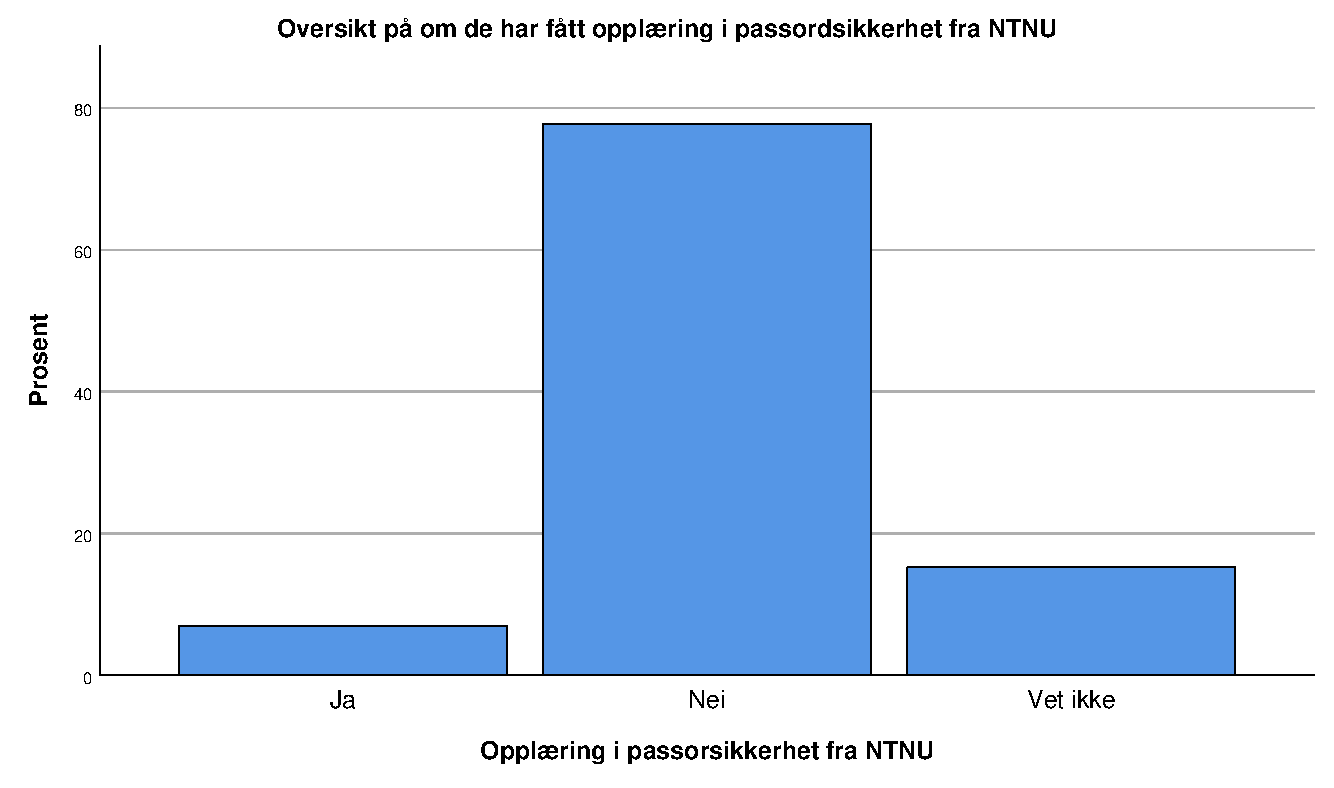
\includegraphics[scale=0.5]{case_2/bilder/spss/opplaring_passordsikk_NTNU.pdf}
    \caption[passordsikkerhet]{Viser hvor mange som har fått opplæring i passordsikkerhet}
    \label{fig:passordsikkerhet}
\end{figure}
Vår hypotese her stemte, de ansatte har ikke fått tilstrekkelig opplæring i passordsikkerhet.  


\subsection{Konklusjon}
Ut fra spørsmålene om bruker- og passordvaner kan vi konkludere med at passordsikkerheten til de kompromitterte er lav. De fleste har brukt sitt NTNU passord på flere tjenester og over halvparten har også brukt sin NTNU e-post på andre tjenester. Dette er mest utbredt på tjenester relatert til jobben. I tillegg til det benytter mange seg av passord som er mellom 8-11 tegn, noe som er rett over minimumsgrensen. De fleste bytter passord sjeldnere enn hvert andre år, selv om retningslinjer for behandling av brukernavn, passord og andre autentiseringsdata \cite{RetnBPA} anbefaler å bytte det hver tolvte måned. 

Noe av årsaken til dette denne lave kompetanse kan være at de ikke har fått tilstrekkelig innføring i passordsikkerhet fra NTNU og IT-reglementet som er krav til at de skal lese igjennom sier lite om bruker- og passordvaner. IT-reglementet sier ingenting om antall tegn på passord eller hvor ofte passordet skal byttes, dette står som en anbefaling fra orakeltjenesten om hva du skal forholde deg til når du lager passord og hvor ofte du skal bytte.   

%----------------------------------------PHISHING---------------------------------
\section{Phishing}
Over 70\% av respondentene sa at de har oppdaget phishing e-post en eller flere ganger på sin NTNU e-post, og rett under 20\% som ikke har oppdaget phishing e-post. Resten av respondentene svarte at de ikke vet. Dette vises i diagrammet under \ref{fig:oppdaget-phishing}.
\begin{figure}[H]
    \centering
    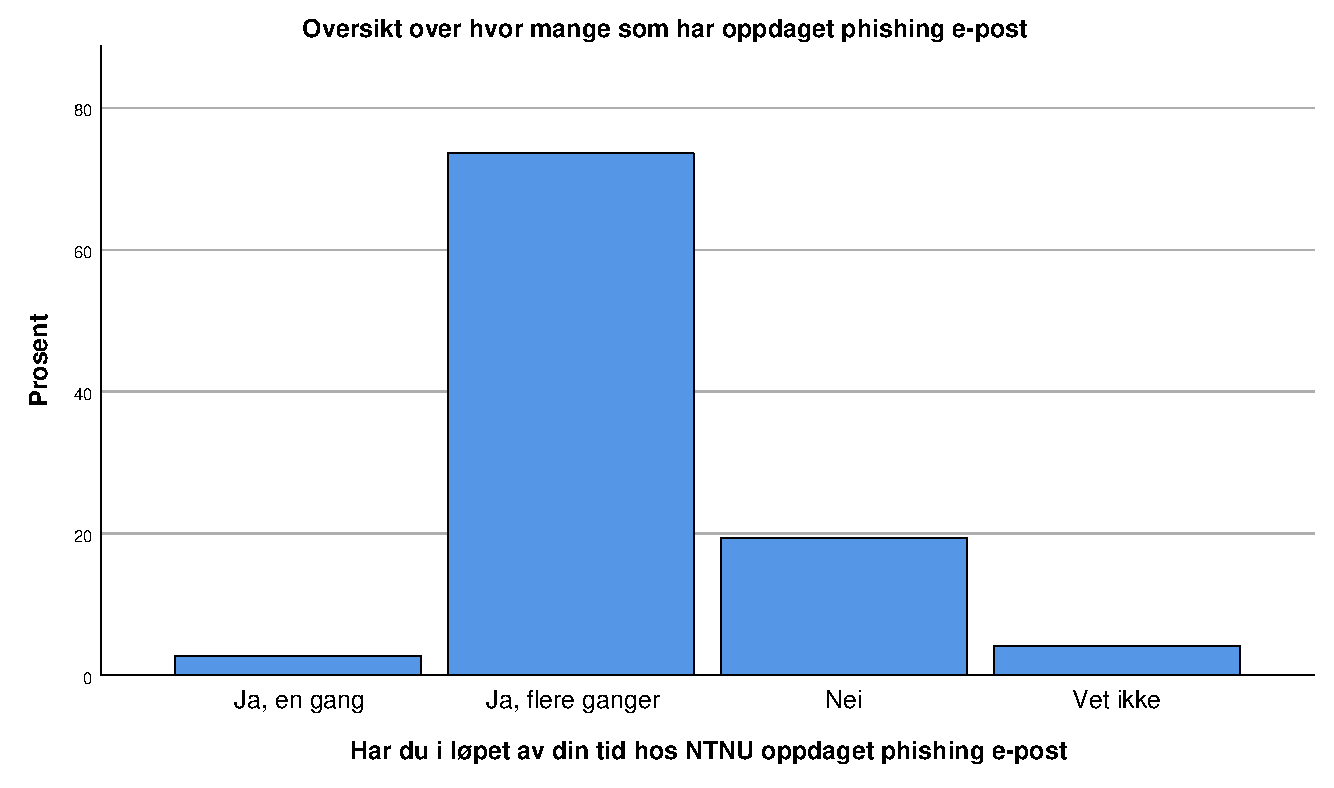
\includegraphics[scale=0.5]{case_2/bilder/spss/oppdaget_phish.pdf}
    \caption[oppdaget-phishing]{Viser hvor mange som har oppdaget phishing e-post}
    \label{fig:oppdaget-phishing}
\end{figure}
Hypotesen vår er sann. Phishing er en svært utbredt angrepsvektor. 

Over 70\% av respondentene sier at de ikke har blitt lurt av phishing e-post, og under 20\% sier at de har blitt lurt. Som vist i tabellen under \ref{fig:lurt-av-phishing}. 
\begin{figure}[H]
    \centering
    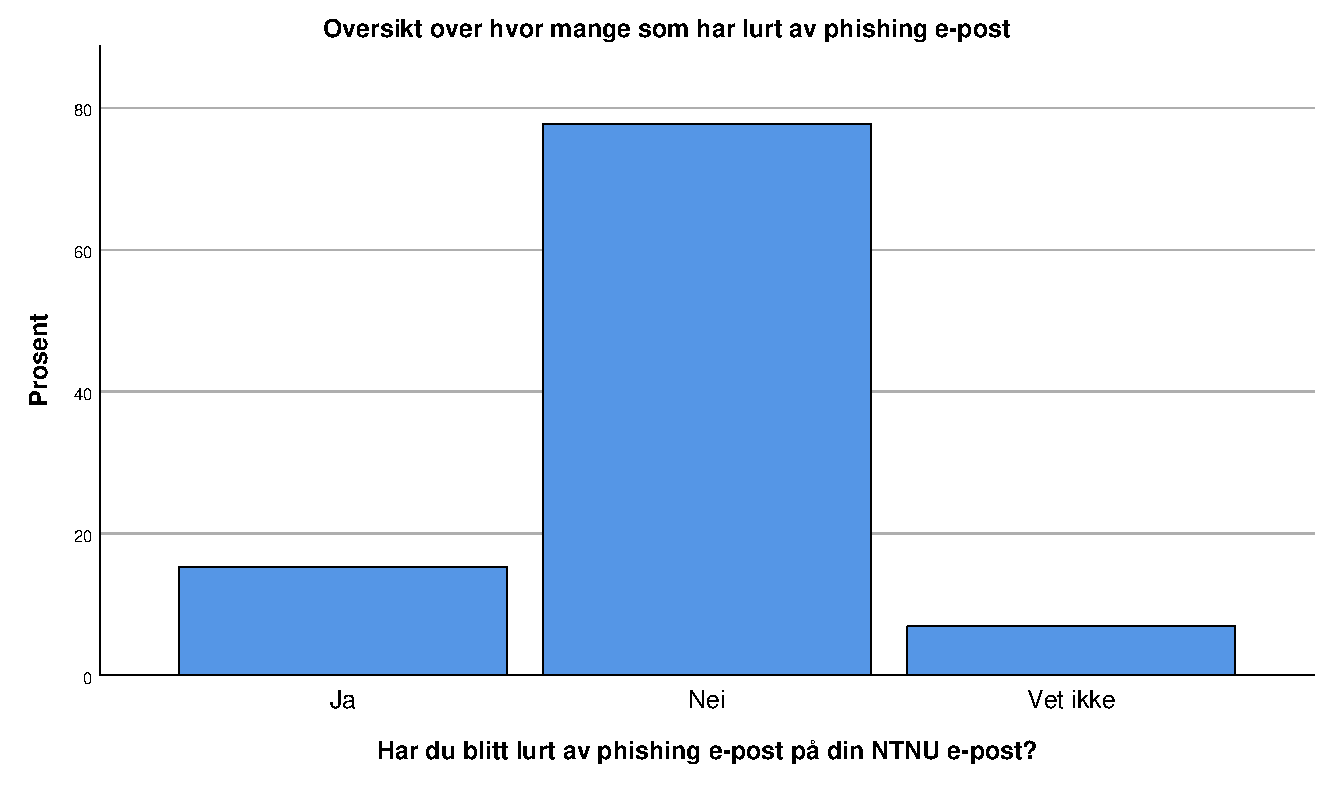
\includegraphics[scale=0.5]{case_2/bilder/spss/lurt_phish.pdf}
    \caption[lurt-av-phishing]{Viser hvor mange som sier de har blitt lurt av phishing}
    \label{fig:lurt-av-phishing}
\end{figure}
Ut fra dataen, kan vi si at vår hypotese ikke stemte.   

\subsection{Konklusjon}


%----------------------------------------STATISTISK ANALYSE---------------------------------
\section{Statistisk analyse}
I denne delen bruker vi statistiske analyseverktøy for å finne relasjoner. De analysene vi fremhever her er de vi anså som mest relevante. De mindre relevante er plassert i vedlegg \ref{vedlegg:statanalys}, og de som enten ble ansett som urelevante eller som hadde lite signifikans har blitt utelatt. Som en generell regel for utføring av analysen har vi valgt et signifikansnivå på: \[\alpha \leq 0,05\]

\subsection{ANOVA på alder mot bevissthet og kjennskap}
Denne testen sjekker om det er signifikans mellom alder på respondenten, og hvor bevisste de er på sikkerhet og hvor godt de kjenner til de ulike retningslinjene og reglementene. Alle spørsmålene er besvart på en skala fra 1 til 6, der 1 er lite bevisst eller kjent, og 6 er svært bevisst eller kjent. I tabellen under beskrives svarene til datasettet som er analysert. 
\begin{figure}[H]
    \centering
    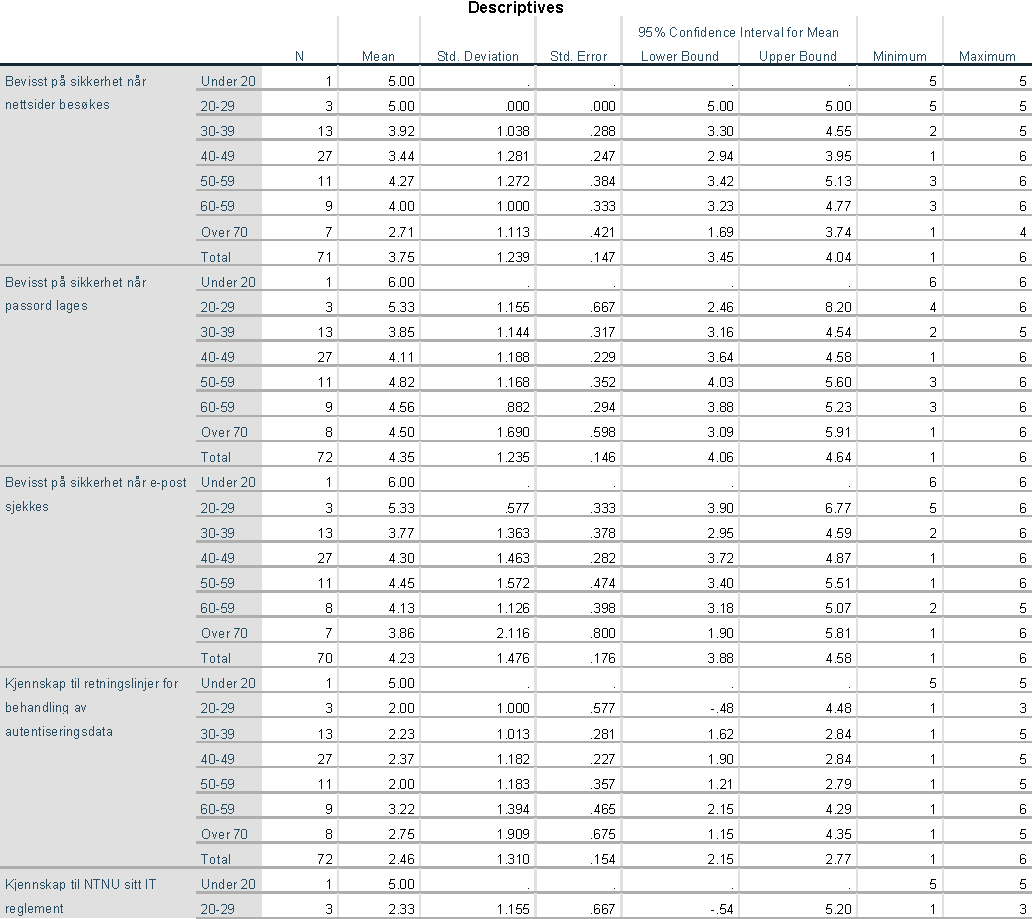
\includegraphics[scale=0.7]{case_2/bilder/spss/anova_ttest/alder_bevissthetogkjennskap_descriptive_1.pdf}
    \caption[alder-bevissthetogkjennskap-descriptive-1]{Descriptive av alder mot bevissthet på sikkerhet og kjennskap til retningslinjer, del 1}
    \label{fig:alder-bevissthetogkjennskap-descriptive-1}
\end{figure}

\begin{figure}[H]
    \centering
    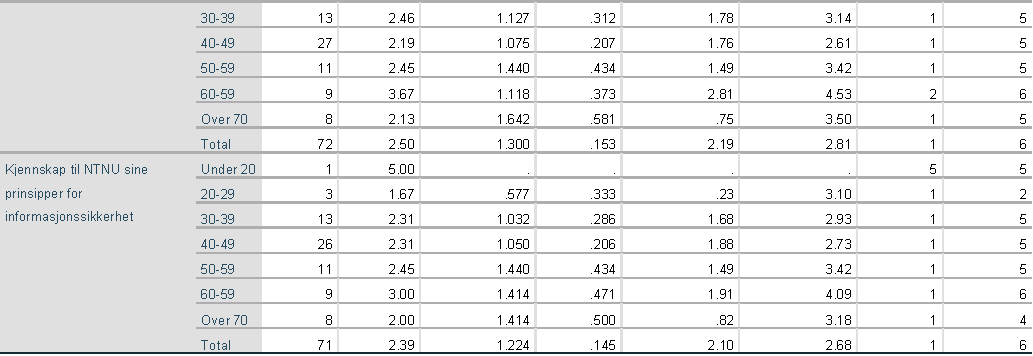
\includegraphics[scale=0.7]{case_2/bilder/spss/anova_ttest/alder_bevissthetogkjennskap_descriptive_2.pdf}
    \caption[alder-bevissthetogkjennskap-descriptive-2]{Descriptive av alder mot bevissthet på sikkerhet og kjennskap til retningslinjer, del 2}
    \label{fig:alder-bevissthetogkjennskap-descriptive-2}
\end{figure}

Fra dataene over kan vi se at generelt sett går bevisstheten på sikkerhet og kjennskapen til retningslinjene ned etterhvert som respondentene blir eldre. Dette gjelder spesielt for bevissthet på sikkerhet når nettsider besøkes og kjennskap til IT-reglementet. 

\begin{figure}[H]
    \centering
    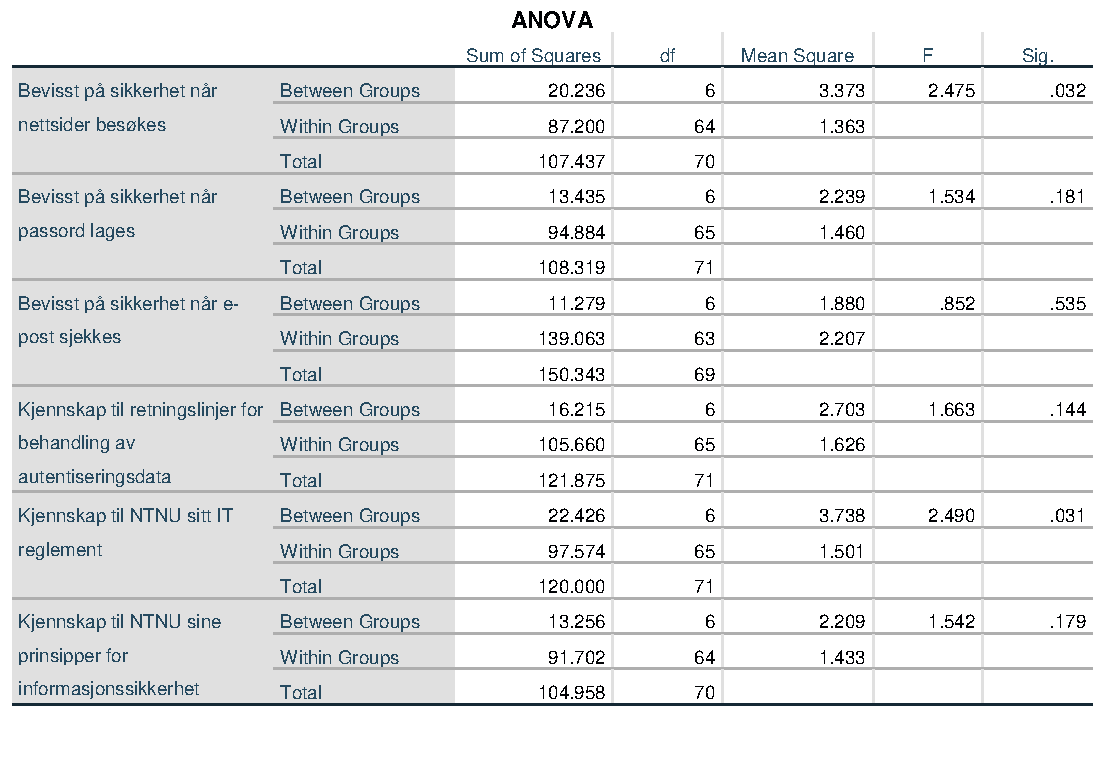
\includegraphics[scale=0.7]{case_2/bilder/spss/anova_ttest/alder_bevissthetogkjennskap_anova.pdf}
    \caption[alder-bevissthetogkjennskap-ANOVA]{ANOVA av alder mot bevissthet på sikkerhet og kjennskap til retningslinjer}
    \label{fig:alder-bevissthetogkjennskap-ANOVA}
\end{figure}

I tabellen over ser vi at når det kommer til alder basert på bevissthet på sikkerhet når nettsider besøkes er dette signifikant siden \(\alpha = 0,032\). Dette betyr at vi kan konkludere med at jo eldre folk blir, jo mindre bevisste er de på sikkerhet når de besøker nettsider. Dette gjelder også for kjennskap til NTNU sitt IT-reglement, der signifikansen er på \(\alpha = 0,031\). 

En post-hoc test kunne ikke kjøres her fordi en av gruppene bare hadde ett svar. 

\subsection{ANOVA på år ved NTNU mot passord-, e-post- og andre brukervaner}
Denne testen sjekker om det er signifikans mellom antall år respondenten har vært hos NTNU, og om de bruker NTNU e-posten sin på andre tjenester, om de har blitt lurt av phishing og om de benytter sitt NTNU passord på flere tjenester. I tabellen under beskrives svarene til datasettet vi skal analysere.
\begin{figure}[H]
    \centering
    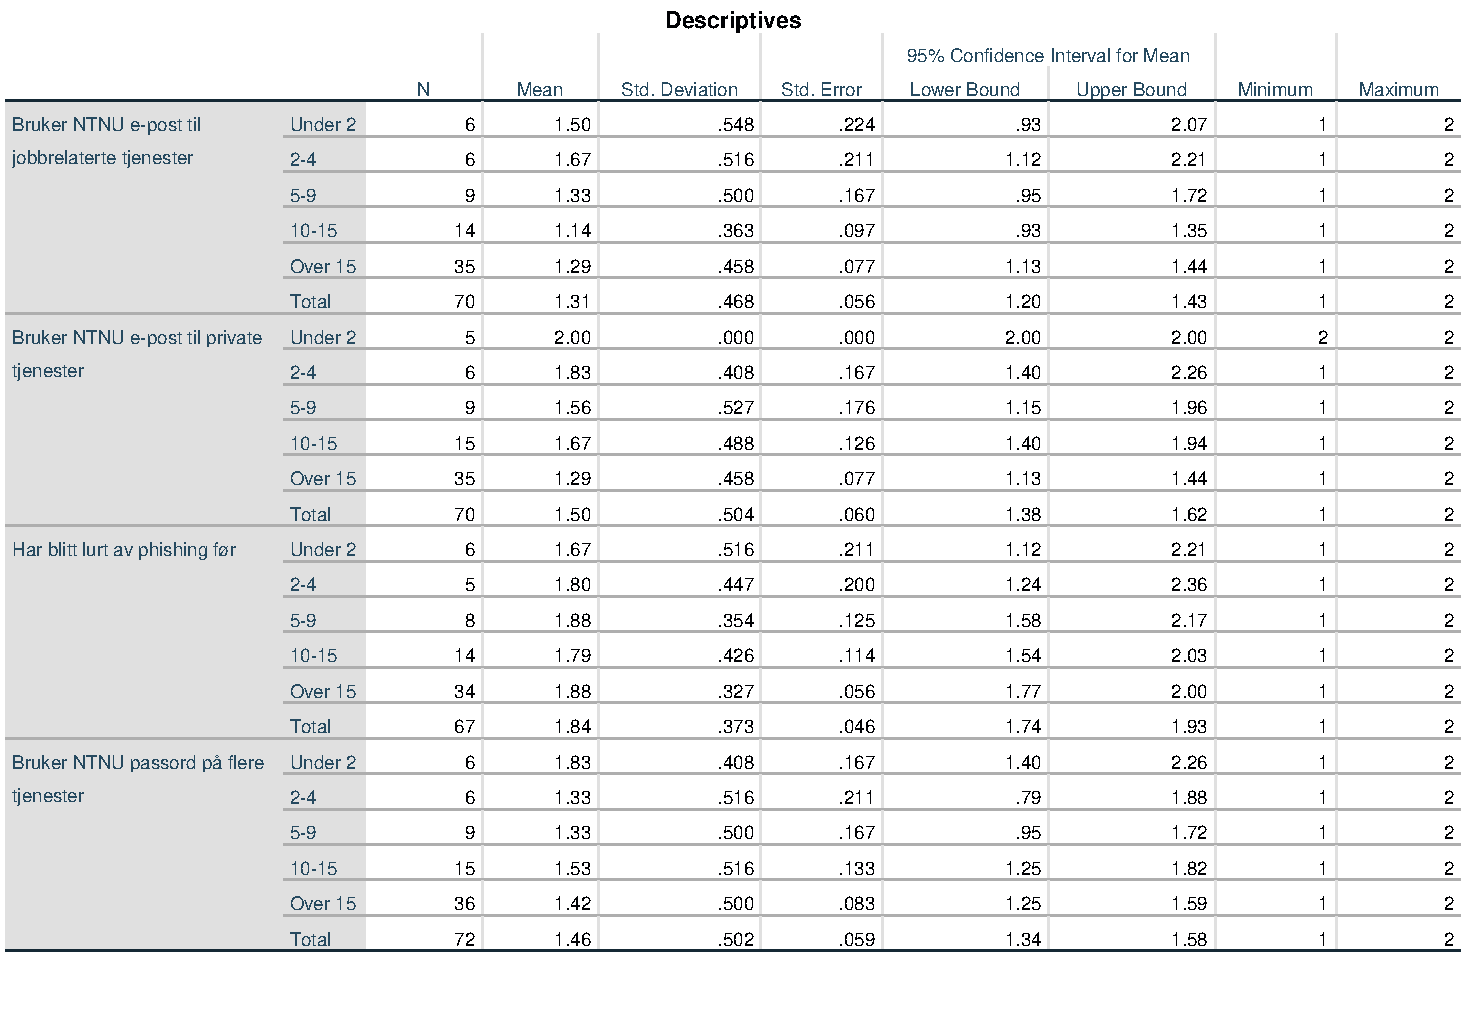
\includegraphics[scale=0.5]{case_2/bilder/spss/anova_ttest/ansiennitet_diverse_descriptive.pdf}
    \caption[ansiennitet-diverse-descriptive]{Descriptive av år ved NTNU mot passord-, e-post- og andre brukervaner}
    \label{fig:ansiennitet-diverse-descriptive}
\end{figure}

\begin{figure}[H]
    \centering
    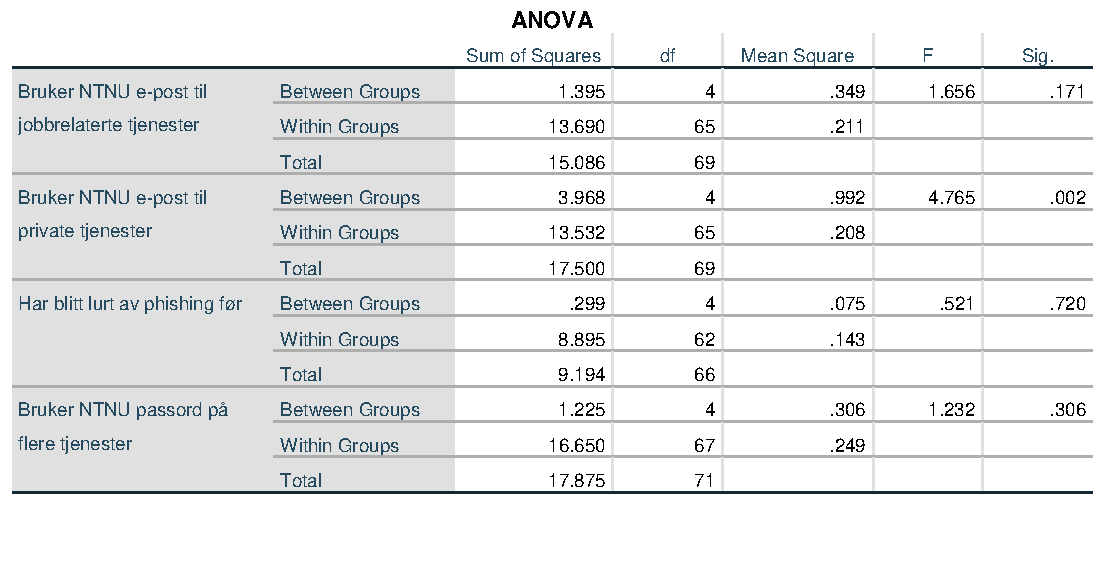
\includegraphics[scale=0.7]{case_2/bilder/spss/anova_ttest/ansiennitet_diverse_anova.pdf}
    \caption[ansiennitet-diverse-ANOVA]{ANOVA av år ved NTNU mot passord-, e-post- og andre brukervaner}
    \label{fig:ansiennitet-diverse-ANOVA}
\end{figure}

Siden det er signifikans på de som bruker NTNU e-post til private tjenester (\(\alpha \leq 0,05\)), ble en post-hoc test kjørt for å se om det var noen ytterligere signifikans mellom gruppene. Grunnet plassbesparelse er bare de variablene som inkluderte signifikans tatt med i rapporten. 
\begin{figure}[H]
    \centering
    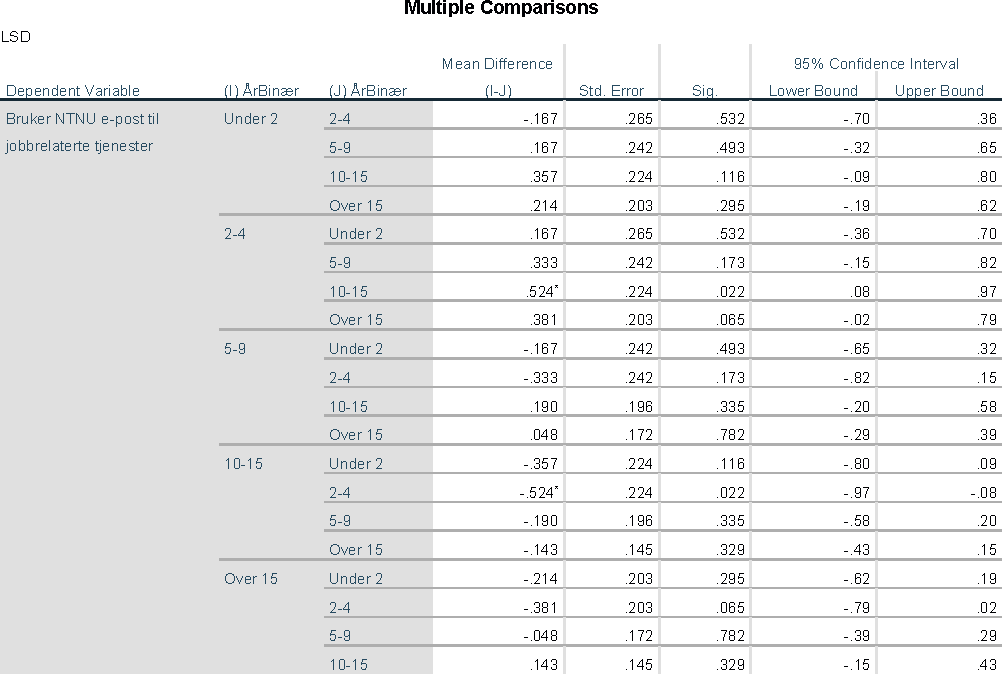
\includegraphics[scale=0.7]{case_2/bilder/spss/anova_ttest/ansiennitet_diverse_posthoc_1.pdf}
    \caption[ansiennitet-diverse-posthoc-1]{Post-hoc av år ved NTNU mot passord-, e-post- og andre brukervaner, del 1}
    \label{fig:alder-bevissthetogkjennskap-posthoc-1}
\end{figure}

\begin{figure}[H]
    \centering
    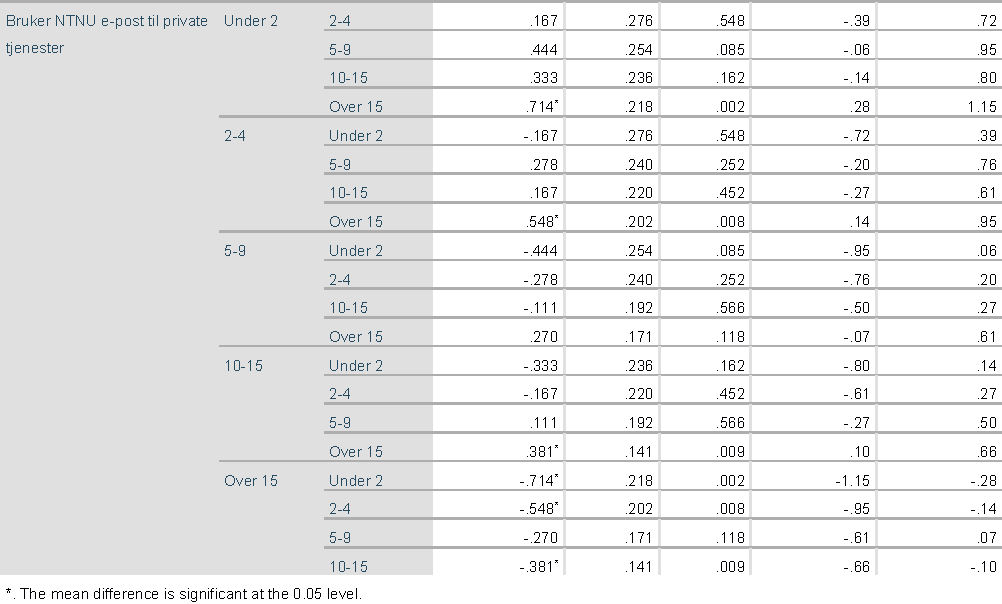
\includegraphics[scale=0.7]{case_2/bilder/spss/anova_ttest/ansiennitet_diverse_posthoc_2.pdf}
    \caption[ansiennitet-diverse-posthoc-2]{Post-hoc av år ved NTNU mot passord-, e-post- og andre brukervaner, del 2}
    \label{fig:alder-bevissthetogkjennskap-posthoc-2}
\end{figure}

I post-hoc testen i figur \ref{fig:alder-bevissthetogkjennskap-posthoc-1} og \ref{fig:alder-bevissthetogkjennskap-posthoc-2} ser vi at når det kommer til jobbrelaterte tjenester er forskjellen signifikant mellom de som har vært ved NTNU i 2-4 år og 10-15 år. Når det kommer til private tjenester er forskjellen signifikant mellom under 2 år og over 15, 2-4 år og over 15, og mellom 10-15 år og over 15. Vi ser at det er en relasjon mellom hvor mange år ved NTNU de og om de bruker NTNU e-post på andre tjenester. Jo lenger de er der, jo mer sannsynlig er det at de bruker e-posten på flere tjenester. 

\subsection{ANOVA på alder mot passord-, e-post- og andre brukervaner}
Siden det ble funnet signifikans på antall år ved NTNU og bruk av NTNU e-post på private tjenester, kunne det være sannsynlig at dette også korrelerte med alder. Det er logisk å tro at jo lenger tid en har tilbringet ved NTNU, jo eldre er personen. Derfor ble det kjørt en korrelasjonstest på alder og antall år ved NTNU for å teste dette. I tabellen under kan vi se at det er en sterk positiv korrelasjon (\(\alpha \le 0,01\)) mellom alder og tid ved NTNU.

\begin{figure}[H]
    \centering
    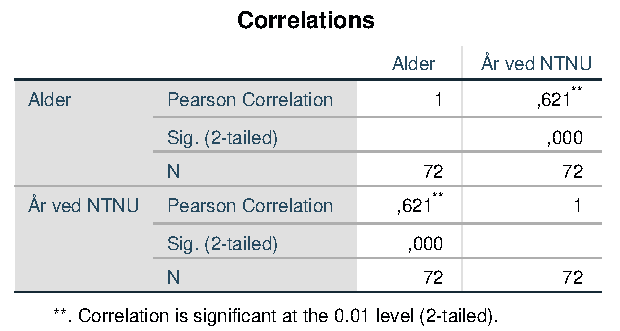
\includegraphics[scale=1]{case_2/bilder/spss/anova_ttest/alder_aarvedNTNU_korrelasjon.pdf}
    \caption[alder-aarvedNTNU-korrelasjon]{Korrelasjon mellom alder og antall år ved NTNU}
    \label{fig:alder-aarvedNTNU-korrelasjon}
\end{figure}

Basert på resultatene er det grunnlag for å tro at siden jo eldre respondenten som har fått sin konto kompromittert er, jo mer sannsynlig er det at personen har benyttet e-posten på private tjenester, basert på resultatene i figur \ref{fig:ansiennitet-diverse-ANOVA} i forrige seksjon.


\subsection{Independent sample t-test på de som har delt passord mot hvor ofte de bytter passord}
Selv om det bare er åtte personer som har sagt at de har delt sitt NTNU passord er dette åtte personer for mye. I IT-reglementet står det at dersom du har mistanke om at noen kan passordet, skal du bytte det med en gang \cite{ITReg}. Derfor var det relevant å se hvor ofte de som har delt passordet sitt bytter passord. Variabelen ``ByttePassordBinær'' går fra 1-4 der 1 er bytte av passord hver sjette måned og 4 er hvert andre år. 

\begin{figure}[H]
    \centering
    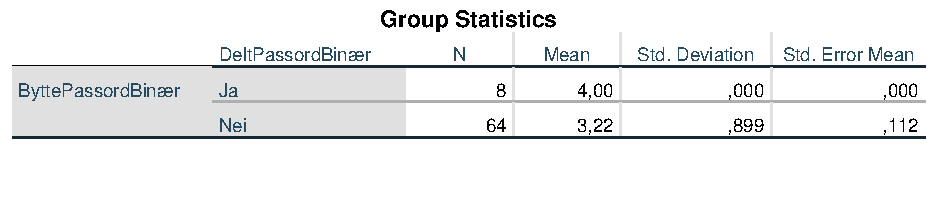
\includegraphics[scale=0.7]{case_2/bilder/spss/anova_ttest/deltpassord_byttepassord_groupstats.pdf}
    \caption[Group statistics av de som har delt passord mot hvor ofte de bytter]{Group statistics av de som har delt passord mot hvor ofte de bytter}
    \label{fig:deltpassord-byttepassord-groupstats}
\end{figure}

Statistikken i figur \ref{fig:deltpassord-byttepassord-groupstats} over viser at alle de som har delt passordet sitt, bytter passord sjeldnere enn hvert andre år. Dette er bekymringsfullt i og med at passordene er kjent av andre over lengre tid. I figur \ref{fig:deltpassord-byttepassord-ttest} sjekker vi om disse tallene er signifikante.

\begin{figure}[H]
    \centering
    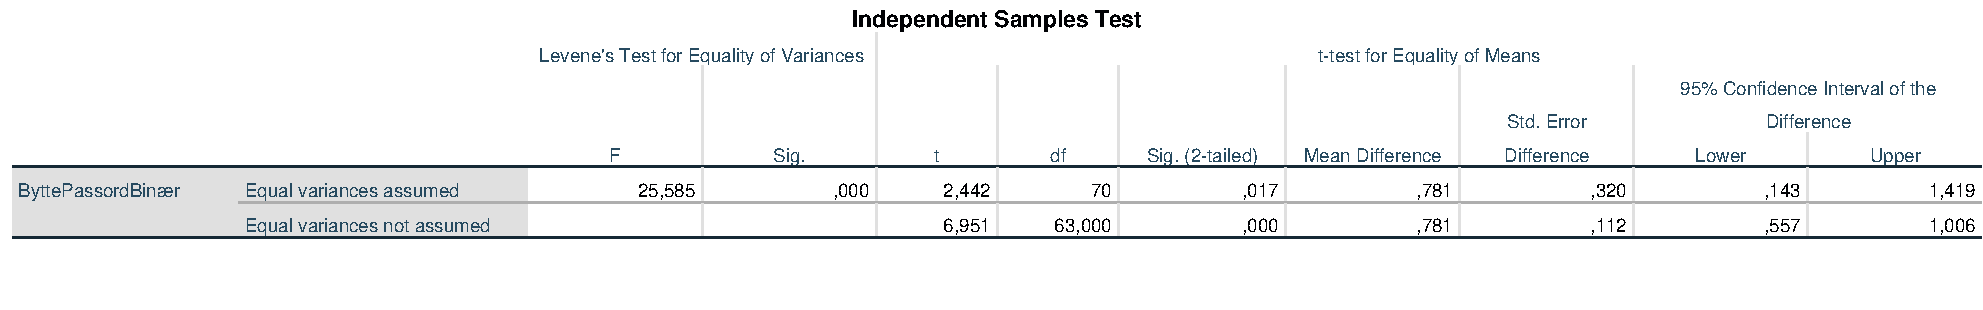
\includegraphics[scale=0.4]{case_2/bilder/spss/anova_ttest/deltpassord_byttepassord_ttest.pdf}
    \caption[Independent t-test av de som har delt passord mot hvor ofte de bytter]{Independent t-test av de som har delt passord mot hvor ofte de bytter}
    \label{fig:deltpassord-byttepassord-ttest}
\end{figure}

Vi kan se at \(\alpha = 0,017\), som betyr at resultatet er statistisk signifikant. 


\subsection{ANOVA på år ved NTNU mot bevissthet og kjennskap}
Det ble ikke funnet noen signifikans mellom gruppene. Det er ingen grunn til å tro at tid ved NTNU har noe til felles med hvor bevisst du er på sikkerhet, eller hvor godt kjent du er med de styrende og rutinemessige dokumentene. Se vedlegg \ref{aarvedNTNU-mot-bevissthetogkjennskap} for ANOVA analysen.


\subsection{Independent sample t-test på kjønn mot bevissthet og kjennskap}
Det ble ikke funnet noen signifikans mellom gruppene. Vi kan dermed ikke si at det er noen forskjell mellom kjønnene av de som har blitt kompromittert, når det kommer til bevissthet på sikkerhet og kjennskap til retningslinjer. Se vedlegg \ref{kjonn-mot-bevissthetogkjennskap} for Independent Sample t-testen. 



\section{Konklusjon av verktøy}
Her så konkluderer vi hvordan vertøyene vi benyttet fungerte og hva som ikke fungerte. 
\subsection{Histogram}
Histogrammer er et velkjent og godt verktøy innen statistikk og fungerer godt i mange forskjellige felt, inkludert rotårsaksanalyse.  Det fungerte også veldig bra i denne sammenhengen for å visualisere problemer knyttet til informasjonssikkerhet, og lettere forstå dataene. Siden dataene ble lettere å forstå førte det også til at vi hadde mulighet til å lage flere histogrammer for å analysere mange aspekter ved spørreundersøkelsen. Det negative med histogrammer er hvis de ulike dataene har stor forskjell på antall respondenter i de ulike kategoriene, kan det være vanskelig å se sammenhenger og korrelasjoner visuelt sett. 

\subsection{Sektordiagram}
Sektordiagram fungerte veldig bra, det var en god måte å illustrere helhetlig fordelingen av respondentene. Det negative med sektordiagram er hvis det er mange svarkategorier, så vil fordelingen kunne bli uleselig. Derfor brukte vi sektordiagram på få kategorier. 

\subsection{Affinitetsdiagram}
Affinitetsdiagram er et vektøy som ikke har sin rot i matematikk eller statistikk, men er heller et mer kreativ verktøy der brukerne bruker sin egen tankegang til å finne de korrelerende gruppene. Dette fungerer bra når dataene man henter er på to forskjellige språk og der deltakerne varierer hvor mye de skriver. Siden dataene er blitt organisert inn i grupper er det mye lettere å analysere hva personene mener er viktig. Det negative med affinitetsdiagram er risikoen for at svarene blir gruppert feil fordi det blir gjort en feiltolkning av hva respondenten mener, eller at det gjøres en feil korrelasjon.    

\subsection{Statistiske analyseverktøy}
Statistiske analyser er fungerte bra, det fungerer veldig bra for å se om det er korrelasjon mellom flere variabler. 

